%% LaTeX2e class for student theses
%% thesis.tex
%% 
%% Karlsruhe Institute of Technology
%% Institute for Program Structures and Data Organization
%% Chair for Software Design and Quality (SDQ)
%%
%% Dr.-Ing. Erik Burger
%% burger@kit.edu
%%
%% Version 1.2, 2016-09-20

%% Available languages: english,ngerman
%% Available modes: draft,final (see README)
\RequirePackage{scrlfile}
\ReplacePackage{scrpage2}{scrlayer-scrpage}
\PassOptionsToPackage{colorinlistoftodos,prependcaption,textsize=tiny}{todonotes}
\PassOptionsToPackage{pdftex,dvipsnames}{xcolor}
\documentclass[english,final,x11names]{sdqthesis}
\usepackage{amsmath}
\DeclareMathOperator\erfc{erfc}
\usepackage[export]{adjustbox}
%\usepackage{menukeys}
\usepackage{array}
\newcolumntype{L}[1]{>{\raggedright\let\newline\\\arraybackslash\hspace{0pt}}m{#1}}
\newcolumntype{C}[1]{>{\centering\let\newline\\\arraybackslash\hspace{0pt}}m{#1}}
\newcolumntype{R}[1]{>{\raggedleft\let\newline\\\arraybackslash\hspace{0pt}}m{#1}}
\usepackage{glossaries}
\usepackage{csquotes}   
\usepackage{xargs}   
\usepackage{tikz,pgfplots}
\usetikzlibrary{calc,patterns,backgrounds, shapes,arrows,chains}
\usepackage{xcolor}
%\usepackage{subcaption}
\usepackage{standalone}
\usepackage[alsoload=binary]{siunitx}
\usepackage[pdftex,dvipsnames]{xcolor}  
\usepackage{chemfig}
\usepackage{mhchem}
\usepackage{xfrac}
\usepackage[font={small}]{caption}
\usepackage{booktabs}
\usepackage{rotating}
\usepackage{pdflscape}
\usepackage{array} 
\usepackage{graphicx} 
\usepackage{placeins} 
\usepackage{subfig}
\usepackage{amsfonts}
\newcommand\lasnotas[1]{\textcolor{red}{#1}}
%\renewcommand\lasnotas[1]{}

%todo-notes:
% \unsure \change, \info \improvement \thiswillnotshow

%custom todo-notes
\usepackage{todonotes}
\newcommandx{\unsure}[2][1=]{\todo[linecolor=red,backgroundcolor=red!25,bordercolor=red,#1]{#2}}
\newcommandx{\change}[2][1=]{\todo[linecolor=blue,backgroundcolor=blue!25,bordercolor=blue,#1]{#2}}
\newcommandx{\info}[2][1=]{\todo[linecolor=OliveGreen,backgroundcolor=OliveGreen!25,bordercolor=OliveGreen,#1]{#2}}
\newcommandx{\improvement}[2][1=]{\todo[linecolor=Plum,backgroundcolor=Plum!25,bordercolor=Plum,#1]{#2}}
\newcommandx{\personalnotes}[2][1=]{\todo[enable,#1]{#2}}

%% ---------------------------------
%% | Information about the thesis  |
%% ---------------------------------

%% Name of the author
\author{Orlando Torres Perales}

%% Title (and possibly subtitle) of the thesis
\title{Integration Technique \\of Photonic Wire Bonding and \\Silicon-Organic Hybrid Devices}

%% Type of the thesis 
\thesistype{Master's Thesis}

%% Change the institute here, ``IPD'' is default
 \myinstitute{Institute of Photonics and Quantum Electronics}

%% You can put a logo in the ``logos'' directory and include it here
%% instead of the SDQ logo
 \grouplogo{IPQlogo}
%% Alternatively, you can disable the group logo
% \nogrouplogo

%% The reviewers are the professors that grade your thesis
\reviewerone{Prof. Dr. Christian Koos}
%\reviewertwo{Prof. B}

%% The advisors are PhDs or Postdocs
\advisorone{M.Sc. Muhammad Rodlin Billah}
%% The second advisor can be omitted
\advisortwo{Dr. Yasar Kutuvantavida}

%% Please enter the start end end time of your thesis
\editingtime{3. March 2017}{3. July 2017}

\settitle

%% --------------------------------
%% | Settings for word separation |
%% --------------------------------

%% Describe separation hints here.
%% For more details, see 
%% http://en.wikibooks.org/wiki/LaTeX/Text_Formatting#Hyphenation
\hyphenation{
% me-ta-mo-delg
}

%% --------------------------------
%% | Bibliography                 |
%% --------------------------------

%% Use biber instead of BibTeX, see README
\usepackage[citestyle=numeric,style=numeric,backend=biber]{biblatex}
\addbibresource{thesis.bib}

%% ====================================
%% ====================================
%% ||                                ||
%% || Beginning of the main document ||
%% ||                                ||
%% ====================================
%% ====================================
\begin{document}
\sisetup{range-phrase=--}
%% Set PDF metadata
\setpdf

%% Set the title
\maketitle

%% The Preamble begins here
\frontmatter

\input{sections/declaration.tex}

\setcounter{page}{1}
\pagenumbering{roman}

%% ----------------
%% |   Abstract   |
%% ----------------

%% For theses written in English, an abstract both in English
%% and German is mandatory.
%%
%% For theses written in German, a German abstract is sufficient.
%%
%% The text is included from the following files:
%% - sections/abstract

\includeabstract

%% ------------------------

%% |   Table of Contents  |
%% ------------------------
\tableofcontents
\listoffigures
\listoftables

%% -----------------
%% |   Main part   |
%% -----------------

\mainmatter

%% LaTeX2e class for student theses
%% sections/content.tex
%% 
%% Karlsruhe Institute of Technology
%% Institute for Program Structures and Data Organization
%% Chair for Software Design and Quality (SDQ)
%%
%% Dr.-Ing. Erik Burger
%% burger@kit.edu
%%
%% Version 1.2, 2016-09-20

\chapter{Introduction}
\label{ch:Introduction}

%%%%%%%%%%% Something something present day communications, bandwidth, etc.
With the proliferation of mobile communications, the amount of internet users has grown exponentially since 1993 to a staggering amount of 2.95 billion users, corresponding to 40.7\% of the world population as of 2014 \cite{ITUinfo15} with an estimated total market penetration of 46.1\% by the end of 2016 \cite{ILSinfo16}. As more devices and users are added to the network, the need for technologies that can support higher data rates has become a key element in the design of server applications and the hardware that supports them. 
\par\medskip
In order to sustain the growth of telecommunication data rates, it is necessary to scale the computation nodes, processing units, datacenters, and most importantly, the links between the interconnected devices. As the bandwidth requirements are increased to handle more users, the volume of data between servers must also be scaled, and the distances that data must traverse without losses become a significant limitation of copper interconnects; Additionally, the Shannon theorem connects the data throughput to the bandwidth of the channel, based on its physical limitations, such as latency and power efficiency. Thus, in order to achieve low power consumption while increasing the data rates, the employment of optical communications has had a great impact in achieving the ever-demanding data traffic in modern short-haul telecommunications. Optica communications feature higher data rates, larger bandwidths and higher noise immunity compared to electrical interconnects, with the additional advantage of reduced complexity of the cabling solutions.
\par\medskip
%$\lasnotas{I still need to connect the speed of data with why optical devices are important}.
%By itself, silicon is an excellent semiconductor candidate for optical communications: Transparent in optical communication wavelengths; highly tunable by doping; and thermally and mechanically stable.
The integration of optical communications to the current state-of-the-art computation nodes demands the use of the existing standardtechnologies in the industry, such as \textbf{silicon-based microelectronics processing}, effectively aligning the well-known processes of microelectronics with new developments in the field of photonics. The concept is extended to the so-called \textbf{silicon photonics}, where photonic platforms are developed using silicon as the core semiconductor component, which provide the technological framework for optical communications compatible with the current microelectronics processing and manufacturing. Silicon is the most widely used semiconductor in the manufacturing of electronics, due to its versatility, availability, low cost, electrical, mechanical and optical properties and industry maturity. Nonetheless, not all of its properties, especially in the optical range, are optimal: silicon is an indirect semiconductor, and possesses a very weak stimulated emission (due to poor radiative band-to-band recombination emission \cite{PavesiSi06}), make it unsuitable as a light emitter, and a lacking an intrinsic electro-optic effect (due to its centrosymmetrical crystalline structure) make it unsuitable for high-speed modulation. Additionally, silicon has better absorption in the UV range than in the deep IR (making it unsuitable for most modern optical communication standards). Thus, additional elements must be integrated to the silicon photonics platform in order to achieve the desired high data rates. 

Since the invention of organic light-emitting diodes (OLED) by Tang and Van Slyke in the 1980s, research in the field of organic semiconductors has flourished and developed substantially \cite{SoOrga09}. Of main importance to the present work are organic semiconductors that can be externally poled leaving a long-lasting polarizability in the molecules conforming the organic compound, making it a suitable electro-optic material, which also has the advantage of possibly enabling direct deposition techniques (such as spin-coating or doctor blading) removing some complexity to the formation of a stack-up formation by crystal growth or lithographic processes, for example. The electro-optic effects are the main focus of study in the present work, by using a silicon-organic hybrid (SOH) platform to provide an alternative to inorganic semiconductor modulation. 
\par\medskip
In the field of microelectronics, the integration process is relatively straightforward, due to the well-established building blocks used in electronic circuits: Resistors, capacitors, inductors and transistors. The building blocks can be easily manufactured by using different materials, such as metals, semiconductors and insulating materials, and thus very diverse electronic circuits can be built and designed for very complex integrated circuits in a single packaged device. In the case of photonic integration, the process must also have basic building blocks which manipulate light such that a specific function is achieved. The photonic building blocks include the light sources, optical amplifiers, optical modulators, polarization circuits, multiplexers, filters and couplers \cite{SmitSiPh14}. Photonic integration may require the use of different platforms in order to exploit the performance of different technologies that could not be otherwise monolithically grown, due to atomic incompatibilities or inherent integration complexity. These devices are the so-called multi-chip modules (MCM), which feature different technologies integrated into a single common carrier. Much like their electrical counterpart, the devices have to connected to each other in order to process light. That means that light must be guided through the connected devices, by means of optical waveguiding or free-space propagation of light. The \textbf{photonic wire bond} (PWB), is of special interest in the context of this thesis as it is the photonic element that connects two optical devices in which light propagates and has small dispersion and low losses with the benefits of the optical range bandwidth inherent in waveguiding. PWBs have the advantage over free-space optical coupling of requiring no active beam alignment, since the PWB is directly attached to the optical device; very stable operation over several temperature ranges; low losses; broadband transmission; and scalability for large-scale device deployment \cite{LindenmannPWB12}. 

%No idea why this is here!
%In the classical model for computing architecture, the transmission, processing and interpretation of information (\emph{software}) has to be done in a physical device (\emph{hardware}). With increasingly complex interconnections and data formatting, the relation between hardware and software has drifted apart from the approach given by Von Neumann in the 1960s into a more complex paradigm. Kirischian \cite{RecCompSysEngKirischian16} distinguishes the role of \textbf{components} as hardware and software, leading to the concept of \textbf{hardware platforms}, which are hardware components designed for a specific implementation.

%The photonic platform building blocks of interest for an optical transmitter consists of one or more of the following elements\cite{USBOpto16}:

%\begin{itemize}
%\item The \textbf{laser} is the optical element that generates the light that is transmitted through the communication channel. The most common communication channel for optical communications are optical fibers.
%\item The \textbf{modulator} is the element that shapes the optical signal (carrier) with the data to be transmitted into the communication channel. The modulator can be a simple, single modulator for on-off keying (OOK) or a group of modulators with more dense data format, such as quadrature phase shift keying (QPSK), by exploiting in-phase and quadrature schemes.
%\item The \textbf{photodetector} is the component that receives the optically modulated signal and correspondingly converts it to an electrical signal. Detection can be done coherently or incoherently depending on the bandwidth availability and the expected signal-to-noise ratio (SNR). 
%\item The \textbf{waveguides} that propagate the light across the different photonic circuits for its manipulation. 
%\end{itemize}


\par\medskip
\begin{figure}[!ht]
\centering
  \includegraphics[width=0.7\textwidth]{visio/Schematic_Concept}
  \caption{Schematic representation of optically- and electrically-packaged transmitter. A laser source is connected through photonic wire bonds (PWB) to a MZM modulator that launches the modulated signal through another PWB to a single mode fiber (SMF). The modulator is driven by electrical wire bonds (EWB) to a printed circuit board (PCB) with RF connectors. The dashed outline shows the optical packaging (in red) and the electrical packaging (in blue).}
  \label{fig:SCH_Concept}
\end{figure}

Figure \ref{fig:SCH_Concept} shows the schematic concept of a fully-packaged transmitter. Without loss of generality, the laser, modulator and output single mode fibers are optically packaged into a single common carrier by using PWBs as optical waveguiding elements. In order to electrically access the device without the need of microprobes, which tend to damage the extremely sensitive devices to mechanical vibrations and external manipulation, an additional electrical wire bonding (EWB) can be added to electrically package the transmitter by means of BNC connectors onto a printed circuit board (PCB) and thus enabling testability and further completely packaging the device. The end product that can be achieved are the so-called active optical cables (AOC)\footnote{https://www.finisar.com/active-optical-cables}, which feature transmitters and receivers optical-based interconnection network. The objective of this master thesis focuses on the optical integration and packaging of the transmitter, specially focused on the process flow steps to achieve a homogeneously-operating transmitter.

%Only the optical packaging is of interest in the framework of this master thesis.

\par\medskip

The master thesis is separated into four main components:
%\footnote{pronounced ``heex-cel'', as its equivalent counterpart VCSELs or ``veex-cels''.};
\begin{itemize}
\item A \textbf{theoretical framework} is provided covering the most important elements that comprise an optical transmitter: The silicon-organic hybrid (SOH) modulator, its theory of operation and important figures of merit; the free-form waveguiding element or photonic wire bond (PWB) and its fabrication principle; and finally, the most important aspects of integrated modulators, such as the light source chosen, featuring a brief introduction to the operation principle of the horizontal cavity surface emitting laser (HCSEL), as well as the optical path losses which provide the most important figures of merit to determine the performance of the optically packaged transmitted.
\item The \textbf{integration process} is described thoroughly, including the variations and discoveries found throughout the experimental procedures. Some elements of past theses are revisited regarding the integration process and the modifications required for a stable process are outlined.
\item The \textbf{data transmission experiment} is used to demonstrate that the multi-chip modules produced are operating adequately. The setups are thoroughly described and the results obtained are discussed. The data transmission experimental setups are described for direct and coherent detection cases. 
%contains the laboratory work and results obtained during the master thesis, including the characterization of the HCSELs; the fabrication process of the transmitter, including the fiber mounting and materials used for the integration; the writing process of the PWBs; the activation of the modulator electro-optical material; and the characterization of the optical modulator. 
%\item The \textbf{discussion} section provides some insights on the obtained results and the thorough analysis of the obtained results. In some cases, the discussion leads to additional laboratory procedures for confirmation of some hypotheses, so some laboratory results are also mentioned here, including the thermal performance of the HCSEL and alternative processing schemes of the transmitter elements.
\end{itemize}

Finally, the outlook of the project and the conclusions are discussed in brief.

%% -------------------
%% | Example content |
%% -------------------


%% --------------------
%% | /Example content |
%% --------------------
%% LaTeX2e class for student theses
%% sections/content.tex
%% 
%% Karlsruhe Institute of Technology
%% Institute for Program Structures and Data Organization
%% Chair for Software Design and Quality (SDQ)
%%
%% Dr.-Ing. Erik Burger
%% burger@kit.edu
%%
%% Version 1.2, 2016-09-20

\chapter{Theoretical Framework}
\label{ch:theoreticalBackground}

In this chapter, the key elements for understanding the theoretical and experimental work that were developed in this thesis are presented. First, the current state-of-the-art of the integration paradigm is presented; next, the elements used in the integration process for the optical transmitter, the modulator and the photonic wire bond, are presented and described. Finally, the most important figures of merit of the optically packaged transmitted are outlined. 

%\section{Preamble}
%\label{sec:thbkgd:pre}

\section{Integration Process Fundamentals}
\label{sec:thbkgd:fmwk}

%As a preliminary step, a few concepts used in the rest of the document are outlined in the following section. %Note that due to space constraints not all the details about each concept are described in here, but only those considered pertinent for the better comprehension of the rest of the document.

The \textbf{platform} in silicon photonics refers to the substrate of a chip architecture, or photonic component, from which the components are constructed. Monolithic platform integration that supports different photonic components, such as light sources and modulators, is greatly simplified when the same platform is shared between components, and in cases where the platforms are physically incompatible, its reliability and long-term stability are greatly hindered \cite{heteroepiCrumbacker98}. 

Conventional microelectronic circuits are grown and manufactured on a silicon platform, due to the relative mechanical and chemical stability of silicon dioxide as an insulator compared to other semiconductors such as germanium \cite{SiGroFisher12}. Analogically, photonic circuits do not necessarily share the same substrate, since the components have specific requirements in which other semiconductor technologies have better performance, and thus additional steps must be taken in order to connect different optical elements that form the fully integrated device, such as a receiver, an optical amplifier, and of special interest for the present work, a transmitter. %Many of the well-known processes of microelectronic circuits manufacturing are preferably employed in integrated photonics. 

The importance of the type of platform used in integrated photonics resides in the ability to realize optical waveguides and other passive optical elements that allow on-chip light propagation with low losses and strong light confinement, with the advantages of the streamlined processing of silicon \cite{ReedSOI92}. \textbf{Silicon-on-Insulator} (SOI) technology replaces the substrate material from thin silicon films to thin insulator films, such as the key element of SOI, the buried oxide (BOX), due to the improved electric parameters, such as low operating voltage and leak current (reduced conductance); high-speed and high-transmission (reduced junction capacitance); and reduced cross-talk, latch-up and high-resistance supporting substrates (full electrical isolation) \cite{FukudaSOI01}, as well as the expected two-dimensional light confinement \cite{SiPhReed04}.
%such as high power consumption and voltage threshold mismatch (leading to increasing gate leakage) under \SI{45}{\nano\meter}, and the related simplifications in System-on-Chip (SoC) architectures and reliability [citation needed].
%As already mentioned in the introduction, the basic components of an optical transmitter are the laser and the modulator. 
\par \medskip
If heterogeneous platforms are used in the construction of photonic devices, some form of optical integration has to be employed between components which cannot have common embedded waveguides, especially important in the case of non-monolithic components, such as physically separated chips. Such processes are not uncommon in microelectronics and are also known as \textbf{multi-chip packages} (MCM), and they have the function of reducing the packaging wiring for high density chips \cite{PolyWong13}. A straightforward approach for optical connections are free-space optical interconnects, which allow for multiple interconnection paths within a specific optical link, by means of diffractive optics \cite{SiPhPavesi16}. One special challenge of free-space optical interconnect is active alignment, since small perturbations (produced by vibration and temperature drift) can cause beam misalignment and thus, loss of the optical link, and by extent reducing the reliability of the system. \textbf{Photonic wire bonding} (PWB) is a novel technique that provides guided optical interconnection between physically-separated chips, which reduces much of the beam alignment complexity of free-space optical interconnects. 
\par \medskip
Much of the work of the Institute of Photonics and Quantum Electronics has focused in recent years in the optimization and analysis of the photonic wire bond, as seen in the works of Lindenmann \cite{LindenmannPWB12} Petek, \cite{IntPWBPetek16}, Rainer \cite{MMIRainer16}, Onanuga \cite{TapWGOnanuga14} and Pakjović \cite{SOHPajkovic16}, among many others, whose contributions provide the foundation of the present master's thesis. 
%\par \medskip
A brief introduction to optical waveguide structures is given in the following, as they form the basis of most of the optical elements discussed along this master's thesis, including the SOH modulators and the HCSELs. 
%For this thesis project, the substrate material of the lasers is an indium phospide (InP) binary semiconductor featuring a zincblende crystal structure, which can be matched by metal-organic chemical vapor deposition in Si(111) with only partial dislocation of 8\% \ref{Krost_InPSilat93}.
%\lasnotas{talk about the quaternary semiconductors here and then about multiple quantum wells} 
%\lasnotas{talk about HCSELs,why they are fantastic for testing, then about integration}
%Nonetheless, it is more practical to characterize and test the elements of the transmitter separately, and hence using PWB as the linking medium between different platforms comes into play. PWBs are manufactured by a two photon absorption (TPA), a nonlinear process which polymerizes a negative-tone photoresist, allowing for free-form shaping of an optical waveguide linking the two optical elements. The advantage of using PWB over other technologies, such as free form lenses, resides in the ease of characterization and streamlined fabrication. 
%The optical path is analyzed from source to transmission endpoint, meaning that the analysis is started at the laser source, the horizontal cavity surface emitting laser (HCSEL), transmitted through the photonic wire bond (PWB), and modulated at the silicon-organic hybrid (SOH) modulator.
%\lasnotas{add more text about the photonic wirebonds}
%The role of waveguides in photonic integrated circuits (PIC) is the same as copper wires in printed circuit boards: to confine electromagnetic signals and propagate them with low loss among the circuit elements for its manipulation and transmission. Optical waveguides can be single-moded or multi-moded, depending on the type of optical signals they carry, and can be analytically solved through Maxwell's equations, and under certain conditions, simplified due to the properties of the medium they propagate through to the Helmholtz equation. %The analytical solution to optical waveguides is broadly treated by Okamoto \cite{OkamotoWG00} and elsewhere in the literature. %Optical waveguides are the foundation of all the optical elements in the transmitter path, as their structural properties provide information on the fabrication requirements and light confinement required at each stage. 
\subsection{Waveguide Structures}
\label{sec:thbkgd:wg}
The structures of the optical waveguides play a very interesting role in integrated optics, since confinement of waves occurs both in the transverse and the longitudinal directions \cite{SelleriWG15}. For a HCSEL, a \textbf{buried waveguide} provides the light confinement necessary for optical gain and lasing process to occur. for optical modulators, the structure is different since it is preferred to allow for an external electric field to manipulate the optical signal: Such structure is the \textbf{strip-loaded waveguide}, which confines the field between two rib structures physically isolated on each side of the confining slot. This allows for an electrode to be mounted on each side of the waveguide, which in turn is used for generating the modulating electric fields through direct contacting using RF microprobes or electrical wire bonding. The driving voltage is reduced compared to other types of structures because of the long interaction length of the electrode and the waveguide, thus requiring less concentration of modulating electric field to change the phase of the optical waveguide. 

\begin{figure}[!ht]
\centering
  \includegraphics[width=0.6\textwidth]{visio/WGarten}
  \caption{Types of integrated waveguides. (a) strip-loaded slot waveguide, (b) rib waveguide, (c) buried waveguide, (d) ridge waveguide. Blue sections represent the high refractive index portion (guiding region). Adapted from \cite{SelleriWG15}.}
  \label{fig:SelleriWG}
\end{figure}
\par\medskip
As already mentioned, since there is no common substrate between the light source and the modulator, photonic wire bonds allow the optical linking of two optically-independent chips. The creation of free-form optical paths has its own challenges, since the symmetry can no longer be assumed and trajectory-dependent losses have an increasingly important role in the assessment of the insertion loss of the device \cite{ToepferPWB14}. Finally, tapers are used to couple strip-to-slot waveguides by confining the optical fields to a region where the guided modes are coupled with low losses, due to its relative large bandwidth, misalignment tolerance, low facet reflections and robustness required for high performance applications \cite{SPThourhout10} \cite{TapWGOnanuga14}. 

%Losses in an optical waveguide originate from scattering, absorption and radiation.

%\lasnotas{Only some of the following topics will be added depending on which are important for the rest of the thesis. Maybe this is unnecesary}

%More on which platforms are promising in SOH OD
% $\Chi^{2}$ NL, TPA, Spont Emi light
% Waveguides
%MZM/IQ
%Figures of merit BW, Pow, Drive voltage
% Functionalization
% Organic Claddings: DDMEBT 4WM, DFG
 %Basic waveguides:
%	Strip, slot, strip-loaded, double-slot
%field-enhancement: E field discontinuity = interaction b/w mode/cladding
 %Strip: easy fab, low O loss 0.2dB/mm, high drv volt
 %Slot: high conf, low TPA (NLO@pow), diff fab (DUV litho, e-beam), 0.7dB/mm vert OK, hor better alas diff
 %strip ld: EO dev, control cladd E field (enhan). Ideal overlap, low volt; Engi (RF,opti loss). FCA. Elaborate fb. (Difficult design)
 %2xslot: disp eng., ph. match w/ 2nd order NL; DFG, SFG. confined, high NL interact $\chi^2$
% STRIP = EOM!

%Strip-slot-conv:
%	low loss (MultPath Interf) 0.13dB
%	electrodes = separation 
% Log taper

%SOH modulator
% MZ modulator phase shift w/ bias
% phase shift vs. swing%
% IQ modulator (nested modulators)

%\section{Free Carrier Absorption}
%Free carriers can move freely inside a band but they require additional phononic or scattering interactions for momentum conservation \cite{OEDakin06}.

% Electro-optical modulator length , coeff, index changes
%interaction factor $\gamma$
%%%NOT THE SAME AS CONFINEMENT FACTOR!
%%%CONF FACT = Ratio pow in activ sect /tot pow (mode)
%%%INT FACT = Ratio pow(mat+E_field)/tot pow (mode)
%%% INT FACT: only E_x!

%% -------------------
%% | Example content |
%% -------------------




\section{Optical Modulators}

\subsection{Principle of Operation}
In the broadest sense, a signal modulator is a device that mixes a carrier signal $s(t)$, which in the present case is a light source, with a modulation signal $m(t)$ that carries the information of interest. This mixing can be achieved by the electro-absorption or electro-optic effects, and can alter the lightwaves in phase or intensity. %Electro-absorption modulators exploit the absorption edge downshifts towards the forbidden gap due to an external field as first analyzed by Franz and Keldysh \cite{HSphotoDagli07}. 

\begin{figure}[!ht]
\centering
  \includegraphics[width=0.8\textwidth]{visio/PM_MZM_IQ}
  \caption{Symbolic representation of different modulator types. (a) shows a phase modulator, (b) shows the Mach-Zender modulator and (c) the quadrature modulator.}
  \label{fig:mods}
\end{figure}

%\emph{phase modulators},
The building blocks for optical modulation are \emph{phase modulators}, \emph{Mach-Zender modulators} and \emph{optical IQ modulators} \cite{SeimetzMod06}. A symbolic representation of each type is shown in figure \ref{fig:mods}. Light is injected to the modulator and split in two equal-power components, and then travel through different optical paths before mixing again at the output. The elements in the optical path will determine the type of the modulator:
%The modulation field overlaps inside the slot and thus transferring the information of the modulation field into the optical field.
\begin{itemize}
\item A phase modulator has an element in the optical path that is controlled by the modulation signal $m(t)$ and induces a relative phase difference $\Delta \phi$ of the output with respect to the input lightwave.
\item A Mach-Zender modulator is made up of two phase modulators where an input wave is split in two different optical paths. Depending on the phase shift introduced on each arm, intensity (or amplitude) modulation can be done on an optical signal, by having constructive or destructive interference at the output of the modulator.
\item A quadrature modulator is made of two MZM in parallel, and features an additional $-\pi/2$ delay for the MZM path in quadrature\footnote{Generally speaking, the quadrature modulator occupies the negative frequencies of the signal spectrum, thus making an efficient usage of the spectral bandwidth.} while the other MZM retains retains the original phase (hence the naming convention \textbf{I}n-phase/\textbf{Q}uadrature). Such configuration allows for different configurations since the carriers of each section are considered orthogonal to each other, and can be used to make better use of the available optical bandwidth.
\end{itemize}

Relative phase difference of the optical signals can be achieved by means of an additional path in one of the arms\footnote{Since the spatial part of the analytical solution of the wave equation reads as $e^{-j\beta z}$, where $\beta$ is the wave vector of the impinging wave.}.One way to achieve a dynamic chance of the path can be achieved by either changing the carrier density of the modulator, or a shift of the refractive index. This can be done by several physical methods: By physical manipulation of the material, such as controlled silicon strain, for instance, nonetheless it requires high voltages to achieve a sufficiently high phase shift. Changing the carrier density through a PN junction or having an electro-optical material which can change its refractive index under an external electric field and thus, leading to a phase change of the optical carrier, are two more efficient methods to produce such optical phase shift. The method that uses plasma dispersion effect\footnote{A change of the real and imaginary parts of the refractive index by means of carrier concentration change\cite{Reedmod05}.}, by using a PIN diode structure around the optical waveguide to alter the density of free carriers, and thus the refractive index and absorption coefficients, are well-known and have been steadily advanced in the literature \cite{ReedSOI14}. However, this implies an inherent nonlinear transfer function which leads to distortion and chirp\cite{LinMZM14}. Integrated optical circuits facilitate the refractive index shift by means of an active electro-optic (EO) material with strong second order non-linearities. An integrated optical phase modulator is based on an optical waveguide in an electro-optic substrate, thus acting as a \textbf{transverse modulator}. An external voltage changes the effective refractive index $n_\text{eff}$ of the waveguide and therefore, the phase of an incoming optical carrier wave. In the Pockels effect regime, the refractive index change can be assumed linear with an external applied voltage across an electrode length $l_\text{el}$:

%The speed of the device depends on the materials used in its fabrication.  %seems like a random out-of nowhere comment in here

%The optical carrier phase can be
%\lasnotas{this needs to be changed around to accomodate for modulation by either method and then introduce SOH.}

\begin{align}
\phi_\text{PM}(t) = \frac{2\pi}{\lambda} \cdot \Delta n_\text{eff} \cdot l_\text{el} \approx u(t)
\end{align}

The necessary voltage for achieving a phase shift of $\pi$ between the two arms is denoted as $V_\pi$. The transfer function\footnote{The ratio of the input and output of an optical modulator.} for single-arm drive is expressed as:

\begin{align}
\frac{s_o(t)}{s_i(t)} = TF(t) = \exp \left( {j\frac{u(t)}{V_{\pi}}\pi} \right)
\end{align}

Where $s_o(t)$ is the output signal and $s_i(t)$ is the input signal. Interference between waves can be exploited for intensity modulation. In other words, the carrier can be turned on (constructive interference) and off (destructive interference) by using two phase modulators being driven by voltages of the same magnitude but equal (or opposite) signs, respectively. This is referred to as a \textbf{push-pull Mach-Zender modulator}. In this configuration, chirp-free amplitude modulation is achieved (because the phase of both arms is preserved at the output) or \emph{balanced} configuration. The transfer function in the push-pull case $TF_\text{PP-MZM}(t)$ can be reduced in this case to: %The transfer function for the DD-MZM for $V_\pi$ phase shift is therefore
%\begin{align}
%TF_\text{DD-MZM}(t) = \frac{1}{2} \cdot \left( e^{j\frac{u(t)}{V_{\pi_1}}\pi} + e^{j\frac{u(t)}{V_{\pi_2}}\pi} \right)
%\end{align}

%\begin{align}
%TF_\text{DD-MZM}(t) = \frac{1}{2} \cdot \left[\exp \left( {j\frac{u_1(t)}{V_{\pi_1}}\pi} \right) + \exp \left( {j\frac{u_2(t)}%{V_{\pi_2}}\pi} \right) \right]
%\end{align}

%For simplification, the $V_\pi$ on both arms will be set to a single value ($V_{\pi_1} = V_{\pi_2} = V_\pi$) %what is the name when you have the same to the left and the right bleh




\begin{align}
TF_\text{PP-MZM}(t) = \cos \left( \frac{\Delta \phi_\text{MZM}(t)}{2} \right) = \cos \left( {j\frac{u(t)}{V_{\pi}}\pi} \right)
\end{align}

The transfer function for power and field can be observed in figure \ref{fig:TF}. The operating point can be chosen at the quadrature point ($V_\pi$, half power transmission, or \SI{3}{\decibel} point, allowing for maximum swing) or at minimum (or maximum) transmission point. If modulation voltage swing is larger than $V_\pi$, it can be seen that there is no significant effect in the transfer function, and thus \emph{overmodulation} occurs \cite{SaeckingerMZM09}. 
%\cite{OptiCommNguyen09}
\begin{figure}[!ht]
\centering
  \includestandalone[width=0.6\textwidth]{tikz/TF}
  \caption{Generalized transfer function for field and power. The power transfer function is cosine-shaped and has the null point at $V_\pi$ or half-wave bias voltage, which is the voltage required to shift the input by $\pi$ at the output port. This point also provides the most linear transfer characteristic and thus its importance in MZM optical characterization.}
  \label{fig:TF}
\end{figure}

\begin{figure}[!ht]
\centering
  \includegraphics[width=0.8\textwidth]{visio/mod_formats}
  \caption{Modulation formats. (a) shows On-off keying (OOK), which can be achieved by simply turning the carrier signal on and off, such as in a MZM. (b) and (c) show quadrature phase shift keying (QPSK) and seno-denary quadrature amplitude modulation, or 16QAM, which use IQ modulators to achieve the data constellation observed in the figure.}
  \label{fig:mod}
\end{figure}

Finally, the modulation formats that are used in this work are shown in \ref{fig:mod}. The simplest modulation format, on-off keying, can be done simply by using a MZM and modulate the amplitude of the carrier. The other two formats exploit the orthogonality obtained in the arms of the IQ modulator and achieve different constellations in the phase diagram that correspond to a different binary value, in this case a 16-bit symbol. 

%An optical carrier is intensity modulated by an RF signal with an MZM biased at quadrature \cite{LeeMZM06}. 

Several figures of merit can be obtained from Mach-Zender modulators which provide a reference for the performance. All modulators present a periodic \textbf{free spectral range} (FSR) which occurs when the constructive and destructive interference at the output reach their maximum value, and so the maximum and minimum transmission is observed. This also provides information on the \textbf{extinction ratio}, which gives the dynamic range of a modulator (i.e. the intensity difference between maximum and minimum transmission), as a function of the effective additional distance traveled by a wave inside the modulator (large path length difference leads to small FSR). It is common in the literature to see these modulators referred to as unbalanced (i.e. optical path imbalance) and balanced (i.e. equal optical paths on both arms). The differential delay of a Mach Zender interferometer can be calculated from the free spectral range as $\text{FSR}=1/\tau$. As mentioned before, $\text{V}_\pi$ also provides information of the first zero of the power transfer function of the MZM, i.e. the linear region operation, which is preferably low in order to use low power for driving the device. Since there is a change of the refractive index of the electro-optical material, phase matching can be of great importance if there is a slight variation of the phase in one of the arms. The bias point of the modulator can be thus shifted to allow for maximum (or minimum) transmission in each arm of the modulator, or for jitter control by using an embedded thermal phase shifter that operates on the basis of a resistor on top of a waveguide that produces an optical phase shift in one on the arms based on Joule heating.

%For most cases, the modulator is considered \textbf{balanced} if the phase between the two arms of the MZM are of equal length. If a length variation is introduced in one of the arms, one can refer to the modulator as \textbf{unbalanced}, which can be corrected if one of the arms can be independently biased to match the phase on both arms. 



%A Novel Measurement Approach for the Half-wave Voltage
%of Phase Modulator based on PM-MZI Photonic Link
%Li Xianghua, Yang Chun*, Ye Quanyi, Chong Yuhua, and Zhou Zhenghua

\subsection{Electro-Optic Effect}
%$\textbf{\epsilon}(\omega)$
The electro-optic effects correspond to the change of the refractive index or absorption coefficient of a material, $\Delta n$ and $\Delta \alpha$, respectively, due to an external electric field. The quantities are closely related through the Kramers-Kronig relations \cite{OEDakin06}. Changes in the refractive index are modeled through the dielectric function $\mathbf{\epsilon}(\omega)$ of the material. From Maxwell's constitutive equations it is known that the displacement vector $\underline{\textbf{D}}$ in an anisotropic medium is proportional to the electric field by $\underline {\mathbf{E}} = \frac{1}{\epsilon_0} \underline{\mathbf{\eta}} \underline{\mathbf{D}}$ in a form that is convenient to represent the \textbf{dielectric impermeability tensor} $\underline{\mathbf{\eta}}= (\epsilon_0 \underline{\mathbf{\epsilon}}_r)^{-1}$. This is widely studied by the field of crystal optics, with the impermeability tensor expanded around $\mathbf{E}=0$ leading to the linear and quadratic electro-optic effects \cite{PhotoSaleh91} as:
%$\underline D = \underline\epsilon_0 \underline\epsilon_r \underline E$



%\begin{align}
%\eta_{ij} (\mathbf{E}) = \eta_{ij} + \sum_k r_{ijk} E_k + \sum_{kl} s_{ijkl} E_k E_l, \qquad i,j,k,l=1,2,3
% \end{align}

\begin{align}
\underline \eta_{ij} (\mathbf{E}) = \eta_{ij} + \sum_k \underline r_{ijk} E_k + \sum_{kl} \underline s_{ijkl} E_k E_l, \qquad i,j,k,l=1,2,3
 \end{align}

Since the dielectric impermeability tensor is proportional to the inverse of the square of the refractive index, the \textbf{electro-optic tensor} $\underline{\mathbf{r}}_{ijk}$ is usually used in the literature to describe the strength of the impermeability tensor under an external field. Due to inherent crystal symmetries \cite{BoydNLO08}, many of the tensor components vanish, leading in anisotropic crystals to strongly preferential $r_{33}$, $r_{13}$ and $r_{63}$ coefficients, depending on which orientation the material of interest is used. For uniaxial crystals, if an optical wave propagates through a crystal of length $L$, the normal modes experience a phase delay $\Delta \varphi = r_{63}n_o^3E_z k_0 L = r_{63}n_o^3 k_0 U$. This configuration is known as a \textbf{Pockels cell}. 

%A reduced electrode length results in a lumped capacitance that limits the bandwidth to approximately \SI{1}{\giga\hertz}, with modulator lengths in the centimeter range. 
%The fabrication of \ce{LiNbO3} wafers can be done by indiffusion in metals \cite{WootenLiNBo300} and can be cut in different directions depending on the applications. In order to achieve larger transmission speeds, ridge waveguides must be used since they confine the electric field in the waveguide better and confines the optical mode more tightly; the challenge in ridge waveguides made from \ce{LiNbO3} relies on the etching and directionality of the waveguide, which in turn determines the confinement quality and thus the losses of the modulator.
The most prominent inorganic material used for optical modulators is lithium niobate, also known as \ce{LiNbO3}, which has been enabled for low driving voltage, low drift and bias-free operation, as well as optical transparency and high electro-optic coefficients \cite{WootenLiNBo300}. A significant disadvantage of \ce{LiNbO3} modulators is that large voltages or long interaction lengths (by means of the electrode length) are required for efficient modulation, thus the figure of merit $V_\pi L$ provides information of the switching capacity of the modulator per unit length. The $r_{33}$ value of \ce{LiNbO3} is \SI{32.2}{\pico\meter/\volt} at \SI{632.8}{\nano\meter}  \cite{BosshardOrgaNLO95}. This provides a good rule of thumb for the expected value in organic compounds, at optical telecommunication wavelengths (\SI{1.3}{\micro\meter} and \SI{1.55}{\micro\meter}), such as SEO100 and SEO250, produced by Luxtera, that have reported $r_{33}$ values of \SI{160}{\pico\meter/\volt}  and \SI{250}{\pico\meter/\volt} \cite{HerreraSEO12} \cite{JouaneSEO14}. Thus it can be seen directly from these that the required driving voltage of a SOH modulator is significantly lower than that of inorganic material, as well as a smaller footprint.

%1. O. Herrera, “Nonlinear Photonics in Waveguides for Telecommunications”, Ph.D. Dissertation, College of Optical Sciences, University of Arizona (2014)
%Y. Jouane, Y-C. Chang, D. Zhang, J. Luo, A. K-Y. Jen, and Y. Enami, “Unprecedented Highest Electro-Optic Coefficient of 226 pm/V for Electro-Optic Polymer/TiO2 Multilayer Slot Waveguide Modulators”, Optics Express, DOI:10.1364/OE.22.027725, (2014)




\subsection{Silicon-Organic Hybrid Modulators}

%LinBO3: photorefractive effect: electrons ionized impurities excited to CB, charge separation, local e field,delta EO effect 
%equivalent resitance due to molduation: conductivity in buffer and EO material. Resistivity control of buffer and match to WG layer before deposition!

%Independent LiNBO3: Anisotropy. TE/TM mode coupling with off diagonal elements of electro optial tensor. Require special crystam cuts and electrode geometries. Not for high speed

At the core of the silicon-organic hybrid (SOH) Mach-Zender modulator (MZM) there are two SOH phase modulators, which consist of a slot waveguide covered by an organic electro-optic material, that are driven in push-pull mode by a single coplanar transmission line in ground-signal-ground (GSG) configuration \cite{Koos_SOH2015}. 

\begin{figure}[!ht]
\centering
  \includegraphics[width=0.7\textwidth]{figs/striploadedWG}
  \caption{Schematic cross section of an SOH MZM showing Si strip-loaded slot waveguides. Two slot waveguide phase modulators, driven in push-pull operation by a single coplanar ground-signal-ground transmission line. The signal is split and combined between the two arms using a multimode interferometer (MMI). The slots are filled with an electro-optic polymer which is poled in a previous step with a voltage $V_\text{pol}$. Below, the simulation of the interacting optical and RF field are shown, showing the strong overlap in the slot region. Adapted from \cite{Koos_SOH2015}.}
  \label{fig:striploadedWG}
\end{figure}

The \textbf{silicon-organic hybrid} (SOH) platform incorporation of organic compounds extend and improve the functionalities that cannot be achieved by silicon alone, and yields a very large amount possible engineering solutions to cater to fully integrated solutions \cite{SOHPICKorn13}. Organic compounds are usually used as the cladding, since the wave interaction that exploits the Pockels effect occurs inside the waveguide slot. The modulating field leads to an ultrafast electro-optic effect with high field overlap, since the modulating field and the carrier are confined inside a very narrow space \cite{gateAlloatti12}. Since the field overlap is very high, the required voltage for strong phase shift is lower than \SI{1}{\volt}. A more detailed schematic description of the physical implementation of the SOH MZM is described in figure \ref{fig:SOHMZMsch}.

\begin{figure}[!ht]
\centering
  \includestandalone[width=0.7\textwidth]{tikz/mzm}
  \caption{Schematic representation of a Mach-Zender modulator (MZM). An input lightwave is split in two equal-power branches by an MMI-based beam splitter, and then converted to an adequate mode field by strip-to-slot converters. An EO polymer is deposited inside the slot waveguides and interacts with the incoming lightwave inside it by an external RF field. The mode fields are re-converted for strip waveguide propagation and recombined in an MMI-based combiner. Adapted from \cite{Koos_SOH2015}.}
  \label{fig:SOHMZMsch}
\end{figure}

The laser light is injected through the input node. For branching the laser light a multimode interferometer (MMI) is used, which is a multimode waveguide optical branch used to split the power into the two arms of the MZM. The preference of MMI for branching power resides on having a simple structure (so there is no need to have an additional structure coupler); large optical bandwidth; polarization insensitivity (as birefringence correction can be used \cite{XipolMMI07}); and robustness against fabrication tolerances \cite{SoldanoMMI95}.

As discussed in the work of Soldano \cite{SoldanoMMI95} and Bachmann \cite{BachmannMMI94}, an MMI can be analyzed through the effective refractive index method to decrease the dimensionality of a 3D problem to 2D. To obtain a 2x2 MMI coupler, and therefore 2 non-mirrored, real images\footnote{Mirroring occurs due to the odd symmetry of the interference, and the real image is also noted because a virtual image is projected into the half-plane $x<0$, but that proves unnecessary for real devices where only forward waves are analyzed.} of a single input field, it is sufficient to have a propagation distance of $z=3L_\pi /2$, which for optical communication yields a value of $\SI{23.5}{\micro\meter} \times \SI{4.5}{\micro\meter}$\footnote{Taken from direct measurement of layout in the IME05 chip}. The same structure would result in constructive interference in one port when mixing the modulated waves incoming from the Mach-Zender interferometer.

%\lasnotas{For this derivation: remember power coupling efficienty for vectorial and scalar fields, mode scalar expansion of a dominant transverse field, itno guided and radiation modes, $\Phi$ is the excitation field, $\Psi$ is the guided mode field or mode field expansion, far from cutoff, resonance condition, $L_\pi$}.

%\lasnotas{The Goos–Hänchen effect (named after Hermann Fritz Gustav Goos (1883 – 1968)[1] and Hilda Hänchen (1919 – 2013)) is an optical phenomenon in which linearly polarized light undergoes a small lateral shift, when totally internally reflected. The shift is perpendicular to the direction of propagation, in the plane containing the incident and reflected beams. It can be shown that the two waves generate an interference pattern transverse to the average propagation direction, $\vec{k}_0 =k(\cos \theta_0 \hat{x}  \sin \theta_0 \hat{z})$ Both waves are reflected from the surface and undergo different phase shifts, which leads to a lateral shift of the finite beam. Therefore, the Goos–Hänchen effect is a coherence phenomenon. See more at \url{http://www.scholarpedia.org/article/Goos-Hänchen_effect}.}

In order to efficiently couple the laser light into the modulator, a strip-to-slot mode converter is employed in order to increase the interaction of the optical field with the cladding to exploit its unique nonlinear optical properties \cite{PalmerSSconv13}. This is achieved through a mode conversion by using tapered waveguides, extensively analyzed in the work of Onanuga \cite{TapWGOnanuga14}.

The optical and RF fields interact inside the slot waveguide and modulation of the optical fields occur because of the application of the RF field by using a ground-signal-ground (GSG) configuration picoprobe and thus achieving a physically achievable push-pull configuration. The waveguide modes are once again converted and recombined by a cascaded slot-to-strip converter and a combiner MMI and finally output to a strip waveguide. 
 
%Double-check if this is important!!!!!!!!!!
%%%%% COCKS %%%%%%%%
%The most important parametrization include the losses from coupling the laser to the photonic wire bond through the taper. The photonic wire bond itself, having a very narrow bend, also induce losses of the laser light. A second taper couples the light to a secondary waveguide which for the interest of the present work acts as a modulator. This can finally be integrated into a full transmitter which can connect to an external processing chip. \cite{IntPWBPetek16}

%\subsection{Silicon-Organic Hybrid Modulator}
%$z=0$
%\begin{figure}[!ht]
%\centering
%  \includestandalone[width=0.6\textwidth]{tikz/lsr+mzm}
%  \caption{Schematic representation of transmitter elements.}
%  \label{fig:SOHMZMschlsr}
%\end{figure}

%\section{Silicon-Organic Hybrid Modulators}
%\label{sec:thbkgd:SOH}



%\subsection{Silicon-Organic Hybrid Platform}
%\label{sec:thbkgd:SOHplatform}


%%%%%%%%%%%%%%%%%%%%%%%%%%%%%%%%%%%% Organic compounds%%%%%%%%%%%%%%%%%%%%%%%%%%%%%%%%%%%%%%%%%%%%%%%%%%%%%%%%%%%%

%\subsection{Poled Polymers}
\subsubsection{Organic Electro-Optic Compounds}
\label{sec:thbkgd:SOHplatform}


Organic non-conjugated polymers can be polarized by an electric field and retain the induced electrostatic charges for a long time, where the electro-physical properties in the polymer system are given by its \textbf{dipole moment}. Highly polar polymers, however, do not have a net permanent dipole moment and have a symmetrical structure. Adding a polar bond into the polymer molecule provides a dipole moment, unless arranged symmetrically (yielding a net zero dipole moment). %This shows that poly(methyl methacryate), poly(vinyl chloride), poly(vinyl alcohol), polycarbonates, and poly(vinlyide flouride) are highly polar materials due to their asymmetric structure, and therefore can have high molecular alignment.\cite{singhmiyataNLOorganic96} \par \medskip

When no external electric field is applied, the dipoles in a polymer are randomly oriented. The dipoles, however, are forced to their random state by intermolecular forces, which can be avoided by increasing the temperature of the polymer, reducing the intermolecular forces, and in this way aligning the dipoles. These polymers are poled through molecular dipole alignment using an external electric field and increased temperature by means of so-called \textbf{thermoelectrets}, possessing a long dipole moment memory, which is important to have long-lasting polymer-based devices that do not require further poling or re-deposition of electro-optic (EO) material. Such polymers can be engineered to improve their optical properties by using a polymer matrix as a guest-host system, or if using covalent bonding by cross-linking the polymer chains, adding as a side chain or adding it to the main chain, as depicted in figure \ref{fig:nlopoly} \cite{GuenterNLO12}, depending on the functional chromophores bonded to the polymer chain. Polymeric materials allow for the possibility to form films by many standard printing techniques (such as spin coating or doctor blading). \cite{BosshardOrgaNLO95}.

\begin{figure}[!ht]
\centering
  \includestandalone[width=0.7\textwidth]{tikz/nlopoly}
  \caption{Types of nonlinear optical polymers. The polymer chain extends along the arrow axis. The donor and acceptor polymers are linked by $\pi$-backbonding. The location of the functional chromophore depends on the linking to the main polymer chain. Side chains are functional chromophores that are linked transversally from the main polymer chain. The functional chromophore can also be located along the main polymer chain. Adapted from \cite{GuenterNLO12}.}
  \label{fig:nlopoly}
\end{figure}
% In 1965, J.F. Ward determined the nonlinear optical susceptibilities by using diagrammatic perturbation theory \cite{NLOPertWard65}, which simplifies the extremely complex algebraic calculation of the polarizability of a material.
Of the previous, for exploiting the Pockels effect, the polymer variants with most promising results are: Polymides with azo chromophores; Methacrylates used as backbones and cross-linked variations; main-chain polyamides; and cross-linked polyurethanes \cite{GuenterNLO12}. In order to find the molecular polarizability of a molecular compound, the full electronic structure of the molecule provides insight on all the possible radiation properties due to polarization in a molecule cell unit \cite{NLOPertWard65}. This is, however, not very practical for increasingly complex organic compounds.
 %The polarizability $\beta$ can be approximated far from resonances as \cite{BosshardOrgaNLO95}: %Another approach exploits instead the fact that for second-order polarizability $\beta$, the dependency is only on strong excitations with low energy  due to charge transfer, leading to the highest occupied and lowest unoccupied molecular orbitals (HOMO and LUMO, respectively) which only depends on the bandgap of the energy levels, the oscillator strength and dipole moment of the charge transfer transition and the laser photon energy, \cite{BosshardOrgaNLO95}
%Some sol-gel systems are currently under research with promising large nonlinearities 
%have good reported performance.
% have good orientational stability and large nonlinearities
%also have large electro-optic effects which are often employed in electro-optic modulators, as well as cross-lined variations.
%are stable and efficient

%defined as: 

%\begin{align}
%\beta_{zzz} (-\omega_3,\omega_1,\omega_2) = 
%\frac{1}{2\epsilon_0 h^2} 
%\frac{\omega_{eg}^2(3\omega_{eg}^2 +\omega_1 \omega_2 -\omega_3^2)}%%
%	{(\omega_{eg}^2-\omega_1^2)(\omega_{eg}^2-\omega_2^2)(\omega_{e%g}^2-\omega_3^2)}
%\Delta \mu (\mu_eg^2)
%\end{align}

%Where the second-order polarizability $\beta_{zzz}$ is a tensor along the charge transfer axis, $\omega_{eg}$ is the transition frequency (which is red shifted due to local field screening effects), $\omega_{1,2,3}$ are the interacting waves, $\Delta \mu$ is the difference between the excited and ground state dipole moments and $\mu_{eg}$ is the transition dipole moment between the excited and ground state (also referred to as \textbf{charge asymmetry}). Far away from all resonances, the dispersion free hyperpolarizability $\beta_0$ along with the case of Pockels effect (where a second wave is not required to interact and the outgoing wave should only be $\pi$-phase shifted, or have a negative sign) yields:

%\begin{align}
%\beta (-\omega, \omega, 0) = \frac{\omega_{eg}^2 (3(\omega_{eg^2}-\omega^2)}{3\omega_{eg^2}-\omega^2)^2} \beta_0, \qquad 
%\beta_0 = \frac{3}{2\epsilon_0 \hbar^2} \frac{\Delta \mu (\mu_{eg}^2)}{\omega_{eg}^2}
%\end{align}
%(EIF model)
Carbon atoms form stable bonds, specifically the $\pi$-bonds which are delocalized electronic charge distributions, allowing for larger mobility of the electron density. Two important parameters, the extent and ease of electron redistribution are measurable by the dipole moment and polarizability, respectively. As stated before, if the charge distribution is asymmetric, the nonlinearity yields a quadratic relation \cite{BosshardOrgaNLO95}. The bandgap and oscillator strength depend on the absorption spectra. Even simpler, the equivalent internal field where the polarizability $\beta$ depends on the length of the conjugated system as $\beta \approx L^3$. An optimal nonlinear optical chromophore has an extended conjugated system, a low energy transition, high extinction coefficient, and a large charge asymmetry, by substitution of the functional groups. \cite{BosshardOrgaNLO95}. Other ways to increase the optical nonlinearities is by adding conjugated bonds (extending the polymer chain) or by substituting the acceptors and donors at the beginning and end of the polymer chain, respectively. Typical characters for donor groups are $p$-like such as amines (with a free electron in the $p$ orbital) and acceptor groups have $s$-like behavior like nitrogen oxide and nitride functionalities\footnote{\ce{NO2} and \ce{-C#N} respectively}. Weak intermolecular bonding has dominant effects in polarizability, which in turn affects the nonlinearities of the molecule. 

%The macroscopic linear approximation of the isotropic model in the weak field regime (!!!!!!this is verbatim!!!!!) can be approximated as $\chi_{333} = 0.2 N\beta^*_{zzz} \mu^*_{g,z} E_p / k_BT$, where $\beta^*_{zzz}$ is the diagonal $z$-element of the hyperpolarizability tensor, $$

\subsubsection{Poling techniques}
\label{sec:thbkgd:poltechs}
%Dye-polymer systems cannot sustain very high electric voltages due to having a low dielectric strength coefficient, making the breakdown electric field an important variable in the poling procedure.
%
The magnitude of second order nonlinearities is related to the dipolar alignment of the molecules; therefore, the poling conditions and the dipole moment of the nonlinear section of the polymer play a substantial role. Nonlinear chromophores are electrically poled at elevated temperatures under an external field nearly at or above the glass-transition temperature by a strong electric field via a technique called \textbf{poling}. The poling process aligns the molecules of the polymer of interest by means of temperature and electric field changes. In order to quantitatively determine the chromophore alignment, the \textbf{ordering parameter} $f$ can be used, with $f=0.30$ as a typical value, with boundary values $0\leqslant f \leqslant 1$\cite{singhmiyataNLOorganic96}. The poling technique depends strongly on the polymer used and the structure containing the organic polymer. In SOH structures, the organic polymer is contained inside the ridge waveguide, and thus \textbf{electrode poling} is the most suitable poling process. %A high-voltage variant, the corona poling, is usually used in thin-film applications or when the sample is exposed. A disadvantage of corona poling lies in surface roughness that leads to optical loss. Using a coating improves this situation by protecting the nonlinear polymers and avoid damage to them.  

%20 non-centrosymmetric crystalline point group materials exhibit piezoelectric behavior, making them nonlinear electro-optic Pockel's effect active.  

%thin-film sample -> sample
A poling temperature for a guest-host system is selected above the \textbf{glass transition temperature} $T_g$ to facilitate dipole rotation and avoid orientational relaxation (i.e. that molecules spontaneously re-align before the poling process is completed). After a predetermined poling time, the sample, still under the influence of an electric field, is cooled down to room temperature, which allows dipoles to remain in a \emph{non-centrosymmetric} polar alignment below  $T_g$ of the composite. This system is known as a ``poled polymer''. %The schematic curve of this process is shown in figure \ref{fig:coronapol}. The poling process steps occur as follows: 

%plot a t2n behavior of the charging current is observed. Such a t2n (n < 1) dependence is a consequence of a ____broad distribution and superposition of relaxation times_____ and is often found in amorphous insulators such as polymers and inorganic dielectrics. These relaxation processes are interpreted as filling of space-charge traps, reducing the driving field at the electrode.

%\begin{figure}[!ht]
%\centering
%\includestandalone[width=0.7\textwidth]{tikz/corona-poling_ALL}
%\caption{Schematic representation of corona poling. Adapted from\cite{singhmiyataNLOorganic96}.}
%\label{fig:coronapol}
%\end{figure}

%\begin{figure}[!ht]
%\centering
%\begin{tabular}{cc}
%\subfloat[]{\includegraphics[width=0.4\textwidth]{tikz/coronapoling}\label{f:cp}} &
%\subfloat[]{\includegraphics[width=0.5\textwidth]{tikz/corona-poling_ALL}\label{f:cpA}} \\
%\end{tabular}
%\caption{Schematic representation of corona poling. \ref{f:cp} shows only temperature, while \ref{f:cpA} shows also voltage and %current applied to the sample. Adapted from\cite{singhmiyataNLOorganic96}.}
%\label{fig:cpol}
%\end{figure}

%\begin{figure}[!ht]
%  \includestandalone[width=0.4\textwidth]{tikz/coronapoling}
%  \centering
%  \caption{Schematic representation of corona poling. $E_p$=Poling field, $T_p$=poling temperature, $T_g$=glass transition temperature, and $T_0$=room temperature. Adapted from \cite{singhmiyataNLOorganic96}.}
%  \label{fig:coronapol}
%\end{figure}

%for which $E_p$=Poling field, $T_p$=poling temperature, $T_g$=glass transition temperature, and $T_0$=room temperature


%\begin{enumerate}
%\item The sample is heated from room temperature $T_0$ to poling temperature $T_p$ and kept at constant temperature and pressure %inside a vacuum chamber.
%\item An external poling voltage $V_p$ (dashed line) is applied at time $t_V$ to the sample, generating a poling field $E_p$%\footnote{The poling field is not shown but it can be extrapolated from the sample width and voltage applied}.%
%\item The sample is cooled to room temperature at time $t_s$ after poling and the electric field is slowly ramped down. 
%\item The thermoelectric treatment generates an electret\footnote{Electrostatic analog of a magnet.}.
%\end{enumerate}

%The corona discharge is a partial breakdown of air at atmospheric pressure, and it is induced by the inhomogeneous electric field around the needle. 
%The corona ions have very low lateral conductivity, so only charges can leak during contact poling.
%Polymers can be crosslinked in order to improve stability over large ranges of temperature, at a set temperature.
%The charge distribution in electrode poling is uniform, but it allows for weaker electric fields than corona poling \cite{singhmiyataNLOorganic96}. 
%no idea what fast charging process is in this context
The electrode poling technique is advantageous because of the simplicity of the setup. The process uses a few volts (and a current within \SI{2}{\nano\ampere} to avoid electric degradation) \cite{BlumPoling98}. The poling technique in-plane gives a large nonlinear coefficient in the TE configuration due to field alignment. The molecular shape and guest-host interactions give the order parameters of a chromophore if there is no preferential orientation (i.e. it is randomly distributed).  Once crosslinking occurs at a specific temperature and the shape can no longer be changed the material is called a thermoset.  %Some crosslinked  polymers change their shape with temperature and cannot dissolve in solvents due to covalent bonding, leading to gelification. This can be overcome by using ionomers which have reversible crosslinking making them suitable for dynamic temperature situations. %By using an angle $\theta$ with respect to the laboratory reference axis, which has a Boltzmann distribution (given by dichroism and electronic distribution).

%Some interesting features can be observed in figure \ref{fig:coronapol}. The poling current behavior follows a $t^{-n}$ dependence \cite{BlumPoling98}

%%%%%%%%%%%%%%%%% Definition of crosslinking
%gelification is a word? 

\subsubsection{Organic material stability}

\begin{figure}[!ht]
\centering
\includestandalone[width=0.5\textwidth]{tikz/temp_dependence_volume_bosshard}
\caption{Temperature dependence of specific volume $V_{sp}$ near $T_g$ from Bosshard, et. al. \cite{BosshardOrgaNLO95}. The cooling parameter $q_1$ shows a linear and a nonlinear (dashed line) cooling rate depending on the properties of the polymer. The phase of the polymer is observed as glass (blue hatched area) and liquid (red hatched area). $T_{eq}$ shows the equilibrium temperature, $T_g$ shows the glass transition temperature and $T_m$ shows the melting temperature.}
\label{fig:Bosshard_temp}
\end{figure}


At high temperatures (above $T_m$, or melting temperature), the organic material is at liquid state (first order transition), with a thermal expansion coefficient (the slope of volume and temperature) $\alpha_l$, and a true equilibrium point at $T_{eq}$ with smaller thermal expansion coefficient $\alpha_g$. The actual phase transition occurs at the glass temperature $T_g$ where the liquid and glass states intersect (i.e. amorphous chain of molecular clusters), and is a kinetic phenomena that depends on the \textbf{cooling rate} $q$ as seen in figure \ref{fig:Bosshard_temp} \cite{BosshardOrgaNLO95}, which shows the measure of the specific volume with respect to temperature. The cooling rate curves are read from a high temperature (above the melting temperature) towards lower temperatures. A cooling rate $q_1$ which is larger than $q_2$ is also shown as well as nonlinear cooling rates, but still the glass temperature point is observed when there is an abrupt change of the thermal expansion coefficient. 

%At $T_g$ the free volume describes the polymer relaxation process, where the total volume is the sum of the free and occupied volumes $v= v_f+v_o$. %$v_o$ is given by the van der Waals radii including the volume associated with vibrational motions. In order to allow movement of molecular segments from one site to another, a critical volume $v_{cf}$ is needed. Considering that liquid expansion of a liquid over the glass state is caused by a thermal expansion coefficient and the free volume at glass transition temperature, 
%A dipolar relaxation time $\tau$ can describe segmental mobility, $r \propto \tau^{-1}$ the WLF equation describes the superposition parameter $a_T$\cite{BosshardOrgaNLO95}.:

%\begin{align}
%log a_T \equiv log \frac{\tau_T}{\tau_\text{ref}} = \frac{-C_1(T-T_\text{ref})}{C_2+(T-T_\text{ref})}
%\end{align}

%Describing also the behavior of viscosity and time-temperature shift factors, with ``universal'' fitting constants \footnote{in the literature it is always suggested to use the fitting parameter at a specific temperature from viscosity measurements} $C_1$ and $C_2$ with typical values for polymers of 17 and 52K. The Vogel-Fulcher formula \cite{BosshardOrgaNLO95}

%\begin{align}
%\tau = A^* e^{B/T-T^*} =  A^* e^{B/T-T_\text{ref} - C_2}
%\end{align}
%(and below $T_g$+\SI{100}{\kelvin}),
At temperatures close to $T_g$, stable behavior of the polymer can be achieved, by heating slightly above the glass transition temperature $T_g$, where maximum mobility of the optical guest molecules occurs. The anisotropy can be fixed by cooling down the polymer with the poling field still on. The shrinking of the specific volume reduces the free space for relaxations of the aligned moieties. This is of special interest to the integration process because the organic polymer is extremely sensitive to temperature, so special care must be taken in the order in which the materials are processed to reduce material instability that will result in overall bad device performance.


%\begin{figure}[!ht]
%\centering
%\includegraphics[width=0.7\textwidth]{figs/BosshardTempDependenceSpecificVolumeNearTg}
%\caption{CORRECT THIS BEFORE PRINTINGGGGG!°!!!!! Temperature dependence of specific volume near %T_g% from Bosshard, et. al.%\cite{BosshardOrgaNLO95}.}
%\label{fig:BehfarRidge}
%\end{figure}

%\section{Solvents (not needed probably)}
%\label{sec:OECompounds:Solvents}

%From wikipedia
%Isopropyl alcohol dissolves a wide range of non-polar compounds. It also evaporates quickly, leaves nearly zero oil traces, compared to ethanol, and is relatively non-toxic, compared to alternative solvents. Thus, it is used widely as a solvent and as a cleaning fluid, especially for dissolving oils. Together with ethanol, n-butanol, and methanol, it belongs to the group of alcohol solvents.

%Auch von wikipedia
%In the semiconductor industry, PGMEA is a commonly used solvent, primarily for the application of surface adherents such as Bis(trimethylsilyl)amine (HMDS) on silicon wafers.

%from http://www.chemicalland21.com/industrialchem/solalc/1-METHOXY-2-PROPYL%20ACETATE.htm

%They may be classified as polar and non-polar. Polar solvents, like water, have molecules whose electric charges are unequally distributed, leaving one end of each molecule more positive than the other. Usually polar solvent has O-H bond of which water (HOH), (\ce{CH3OH}) and acetic acid (\ce{CH3COOH}) are examples. Propanol, butanol, formic acid, formamide are polar solvents. Polar solvents are hydrophilic but non-polar solvents are lipophilic. Polar reactants will dissolve in polar solvents. Non-polar solvents dissolve non-polar compounds best. Oil and water don't mix but separate into two layers. There are three measures of the polarity as "dipole moment", "dielectric constant" and "miscibility with water". Though low dipole moments and small dielectric constants indicates non-polar solvents, sharp boundaries between polar and non-polar solvents are not available. The polarity reflects the balance between a polar component (OH) and a non-polar hydrocarbon component, existing in the same molecule. If hydrocarbon character increases relatively, the polarity decreases. On an operational basis, solvents that are miscible with water are polar.

%\textbf{The appropriate solvent should be selected based on the inactivity in the reaction conditions, dissolving the reagents as well as reactants, appropriate boiling point and easy removal at the end of the reaction.}

%\dots

%\section{Information Theory}
%\label{sec:InfoTheory:InfoTheory}

%\begin{figure}[!ht]
%  \includestandalone[width=0.3\textwidth]{tikz/gaussianchannel}
%  \centering
%  \caption{The Gaussian channel. Adapted from \cite{ThomasInfoTheory91}.}
%  \label{fig:gaussianchannel}
%\end{figure}

%%%%%%%%%%%%%%% RANDOM BOSSHARD QUOTES




%% ---------------------
%% | / Example content |
%% ---------------------


%\section{Solvents and Material Processing}
%\label{sec:solv:solvs}
%Wu states that "Water-soluble polymers can form hydrogels aftercrosslinking. The hydrogel is usually insoluble, butcan absorb considerable water and swell. The swelling ratio [...] strongly depends on the intrinsic properties of corresponding linear polymer, such as solubility and conformation. High solubility and ex-panded conformation in certain solvents lead to a high swelling ratio." \ref{Wu_Solv04}



%\subsection{Organic Electro-Optical Material Characterization}
%\label{sec:EO_optim}

%\lasnotas{probably not necessary}

%It is common to find much higher $r_{33}$ coefficient materials in the literature in very specific laboratory conditions, with comparable coefficients to \ce{LiNbO3} in dedicated SOH structures. In order to characterize electro-optical crystals the half-wave voltage $V_\pi$ is an important parameter, as it indicates the voltage required to obtain a $pi$ phase shift in the transmitted beam in a modulator:

%\begin{align}
%V_\pi = \frac{\lambda}{(n^3r)_\text{eff}\frac{d}{L}=v_pi \frac{d}{L}} 
%\end{align}

%With $(n^3r)_\text{eff}$ being the effective electro-optic coefficient. 




%% LaTeX2e class for student theses
%% sections/content.tex
%% 
%% Karlsruhe Institute of Technology
%% Institute for Program Structures and Data Organization
%% Chair for Software Design and Quality (SDQ)
%%
%% Dr.-Ing. Erik Burger
%% burger@kit.edu
%%
%% Version 1.2, 2016-09-20

%\chapter{Modulators and Waveguides}
%\label{ch:MW}

%In this chapter some elements of modulators and waveguides are provided. In many cases results are only provided instrumentally as they are not the focus of study in the present work, but references for further theoretical foundations are provided.
\clearpage
\section{Photonic Wire Bonds}

Photonic wire bonds (PWB) are optical waveguides based on polymers that interconnect different chips, much like wire bonding being a standard electrical connection technique in electrical integrated circuits. The PWB has a rectangular cross section of $\SI{1.4}{\micro\meter} \times \SI{1}{\micro\meter}$ which satisfies single-moded operation \cite{ToepferPWB14}.

\begin{figure}[!ht]
\centering
  \includegraphics[width=0.6\textwidth]{figs/PWB_fab}
  \caption{Fabrication of PWB, illustrating the process of the connection. Two physically separated chips are placed in common submount, and a negative photoresist is added between the devices. Laser light polymerizes the photoresist by two-photon absorption. Adapted from \cite{ToepferPWB14}.}
  \label{fig:PWB_fab}
\end{figure}

As any other optical path, PWBs introduce losses due to material, bending and transition losses. The polymer losses account for \SI{3}{\decibel / \centi\meter} for $\lambda=\SI{1550}{\nano\meter}$; while bending losses are entirely path-dependent, they can be dynamically calculated when the PWB is written, while in general small curve radii most be avoided when writing PWB; Results from T{ö}pfer suggest a loss of \SI{0.24}{\decibel/\micro\meter} \cite{ToepferPWB14}. 

The material of which PWBs are made of is the negative-tone photoresist IP-Dip produced by Nanoscribe, catered for immersion and drop-casting processing. As any other polymer, the photonic wire bond should have a number of properties that match the pre- and post-processing of a multi-chip package, being the key properties \cite{PolyWong13}:

\begin{itemize}
\item \textbf{Optical properties:} The polymer must have a refractive index that allows for strong waveguiding with low losses. Additionally an overcoating can be used to match the refractive index and reduce return losses due to Fresnel reflections.
\item \textbf{Thermal properties:} The glass transition temperature must be high enough that the material will be stable over the range of temperatures in which the multi-chip module is processed. 
\item\textbf{ Mechanical properties:} The polymer used for the PWB must have a low thermal coefficient of expansion such that, throughout the many processes of the multi-chip module, there will be no warping or delamination of the PWB.
\item \textbf{Solvent resistance:} When the PWB is developed it should withstand different solvents used to remove the regions that are not polymerized. This also introduces a strain due to drying, which can be externally controlled by methods such as critical point drying to avoid uneven strain in the PWB.
\end{itemize}

%presents a glass transition temperature, which has to be taken into account during the thermal processing during device integration. 
The characterization of the PWB is done by measuring the optical paths available on-chip in which there is a well-known optical path. The SOH chips used throughout this master thesis have independent optical paths which allow for independent measurement of the transmission through the input or output PWB and grating couplers for measuring the transmission of the modulator only. The details of the measurement are provided in section \ref{sub:OPL}.

%\section{Photonic Wire Bonds}
\subsection{Fabrication Process}
\label{ch:th:fabPWB}

\begin{figure}[!ht]
\centering
  \includegraphics[width=0.9\textwidth]{figs/pkgprocess}
  \caption{PWB fabrication steps.}
  \label{fig:SOHpkg}
\end{figure}

Photonic wire bonds are not necessarily symmetric in a device since the path it follows depend on the location of the chips, especially when the processing of the chip is done manually. Nonetheless, the chip alignment is not as critical when the dimensions of the chips and components is well known and can be controlled prior to the writing of the PWB. and just determines the losses of the PWB. The fabrication process of the photonic wire bonds is illustrated in figure \ref{fig:SOHpkg}:

\begin{enumerate}
\item The components are placed on top of a common carrier, fabricated in-house, made with aluminum. The components are passively aligned by hand and glued with thermally-curable epoxy. 
\item The IP-dip photoresist is dispensed on top of the common carrier, making sure there is enough photoresist in the region of interest (i.e.between the SOH and the HCSEL).
\item The module is placed in the printing machine and the position of the HCSEL and SOH is found using the software. The structures on-chip that allow for localizing the emission window, tapers and fibers.
\item The waveguide structure is calculated based on the chip distance, relative height, and after inspecting the geometry as a 3D model, the final shape is selected.
\item The PWB is written by polymerization of the IP-dip through two-photon absorption. 
\item After all the required PWB are written, the PWB is developed and prepared for local deposition of the electro-optical polymer.
\end{enumerate}

\subsection{Photonic Wire Bond Stability}

\begin{figure}[!ht]
\centering
  \includegraphics[width=0.9\textwidth]{figs/PWB_stab}
  \caption{PWB stability test. (a) shows the setup, consisting of a hot plate used to control the temperature of the metallic submount in which an SOI is integrated with an overcladded PWB. Figure (b) shows the average PWB transmission in dB for different temperatures and conditions. A standard control measurement in air is taken, and different temperature steps and thermal exposure times are also pictured.}
  \label{fig:SOHtherm}
\end{figure}

The thermal and mechanical stability of the photonic wire bond are of great importance during the integration process since it determines the reliability of its function throughout the lifetime of the optical transmitter. Such study has been addressed by doing thermal stability testing on a functional PWB in a test structure as shown in \ref{fig:SOHtherm}. The setup is a simple hot plate that controls the temperature of a mounted SOI/PWB combined chip, and the transmission on-chip is measured after thermal exposure of the chip. The PWB retains a stable transmission at thermal exposure of more than 60 minutes at \SI{165}{\celsius} and more than 5 minutes at a temperature \SI{250}{\celsius}, thus the reliability of the PWB under laboratory conditions is confirmed for temperatures up to \SI{250}{\celsius}. Further application of heat reaches the glass transition temperature of the IP-dip polymer, which in affects its mechanical stability and causes collapsing of the PWB (thus losing the intended optical path) or in the worst case scenario, detachment from the tapers and inoperability of the device.



\section{Integrated Transmitters}

Even though optical modulation can be done directly in some laser diodes, the most reliable method at high transmission speeds is still external modulation, since it provides with larger degrees of freedom in terms of chirp control, bandwidth and distortion \cite{WootenLiNBo300}. 

The integration of the optical modulator to the optical source is of crucial importance in the miniaturization of devices, since the dimensions of each must be mutually matched in order to accommodate mechanically in a shared common carrier. 

%\subsection{Figures of Merit}
\subsection{Horizontal Cavity Surface Emitting Laser} 

In order to create a semiconductor laser, a resonator structure must be integrated into a very small form factor. To achieve this, a distributed Bragg reflector (DBR) can be used, which consists of a stack of waveguides, in which several partial reflections of an optical wave occur. This leads to a selective photonic passband and thus, acting as the optical cavity of a laser. In order to allow for optical confinement, two n- and p-doped semiconductor layers acting as mirrors are added to an optically active layer, which is known as an \textbf{edge-emitter laser}. If an additional mirror is added at the emission window, and total reflection occurs, the laser beam is emitted vertically, and thus, the basic structure of a horizontal-cavity, surface emitting laser (HCSEL) is achieved \cite{Eichlerlaser15}. %Additionally they are easy to test and package and build. 


%BH_LO_Swingler
\begin{figure}[!ht]
\centering
\begin{tabular}{cc}
\subfloat[Vertical cross-section adapted from \cite{SwinglerThermal14}]{\includegraphics[width=0.4\textwidth,valign=m]{figs/BH_LO_Swingler}\label{fig:RidgeSwingler}} &
\subfloat[Horizontal cross-section adapted from \cite{MoehrleHCSEL10}]{\includegraphics[width=0.5\textwidth,valign=m]{visio/HCSEL_LO}\label{fig:HCSEL_LO}}  \\
\end{tabular}
\caption{HCSEL structure and stack-up.(a) shows a vertical stack-up of a typical InP-based buried heterostructure, featuring conductive metallic layers at the bottom for electrical interconnections, and several InP n- and p-doped layers surrounding the active region at the core of the heterostructure, (b) shows a horizontal stack-up showing details of the active layer and gratings used, as well as the location of the outcoupling mirrors and the contact types. }
\label{fig:HCSELdims}
\end{figure}

%\begin{figure}[!ht]
%\centering
%\includegraphics[width=0.7\textwidth]{figs/Ridge_fromBehfarHCSEL05}
%\caption{Cross-sectional and perspective views of a HCSEL, taken from Behfar, et. al.\cite{BehfarHCSEL05}.}
%\label{fig:BehfarRidge}
%\end{figure}

%\begin{figure}[!ht]
%\centering
%\includegraphics[width=0.6\textwidth]{visio/HCSEL_LO}
%\caption{HCSEL stack-up, adapted from \cite{MoehrleHCSEL10}.}
%\label{fig:HCSEL_LO}
%\end{figure}

The work of Behfar \cite{BehfarHCSEL05} and Moehrle \cite{MoehrleHCSEL10} for the structural and specific dimensioning of the HCSEL were used as a reference for this thesis. A ridge waveguide structure is used for the confinement of light in the lateral region, because of the slight change of the refractive index under the ridge with respect to the etched part, thus achieving weak guiding. Strong guiding structures are not usually used because the edges of the optical core can be actively damaged by a deep etch. Narrow ridges are used for single-lateral mode operation and to the mode matching of the laser to the waveguide \cite{ZappeLaser04} (in this case, the size of the PWB).  The \SI{45}{\degree} angle prevents the ridge structure from interfering with the beam shape \cite{BehfarHCSEL05}. Figure \ref{fig:HCSEL_LO} shows the stack-up structure of a HCSEL buried structure. The HCSELs used in this master thesis are multi-quantum well \ce{InP}. For the emission window, \SI{45}{\degree} facet mirrors are used to emit light vertically.  %An additional monitoring photodector is added after the DBR for power metrology, and it features a Brewster angle-cut facet to avoid back reflections \cite{BehfarHCSEL05}.%Not necessary to talk about the monitoring photodetector
%Analysis

%In order to obtain the dimensions of the laser, a reference image is used from the first SEM pictures and using the image processing software ImageJ. \ref{fig:HCSELdims} shows the approximate dimensions of the ridge waveguide made for the HCSEL. 

\begin{figure}[!ht]
\centering
\begin{tabular}{cc}
{\subfloat[SEM picture]{\includegraphics[width=0.4\textwidth,valign=m]{SEM/laser_MCM01}\label{SEMlaser}}} &
{\subfloat[Schematic dimensions]{\includegraphics[width=0.5\textwidth,valign=m]{visio/HCSEL-dim_v2}\label{HCSELdim}}}  \\
\end{tabular}
\caption{HCSEL dimensions. \ref{SEMlaser} shows the SEM image of the HCSEL. \ref{HCSELdim} shows the image analysis-calculated dimensions from the SEM picture.}
\label{fig:HCSELdims}
\end{figure}

The HCSELs are packaged in arrays of four units. In general, an array of 2 HCSEL arrays (total 8 units) was tested for MZM modulators, while a single HCSEL array was sufficient for IQ modulators. In order to measure quantitatively the performance of a HCSEL array, one expects it to behave predictably at a specific temperature with a constant output power, high side mode suppression ratio and single longitudinal mode operation. Depending on the level of maturity of the laser, the characterization properties are changed in priority with respect to their importance at the system level.
%What limits the maximum output power of ong wavelength InP laser diodes
%verbatim! from  http://citeseerx.ist.psu.edu/viewdoc/download?doi=10.1.1.589.9034&rep=rep1&type=pdf
%for my laser !!!!!strain compensated MQW InGaAsP/InP layer structure!

\subsubsection{Laser Requirements}

The L–I roll-off is typical for laser diodes and it is attributed to self-heating of the device in CW operation. Temperature elevation affects a number of key physical mechanisms in laser diodes, including the optical gain, optical losses, and nonradiative recombination mechanisms [find citation here]. 

In order to use high order modulation formats (as those used in IQ modulators, for example), the laser linewidth has an increasingly important role. In a time period $\tau$, the laser phase noise has a change of $\Delta \phi(t)= \phi(t) - \phi(t-\tau)$  and variance $\left< \Delta\phi^2(t) = 2\pi(\Delta \nu \tau) \right>$, where $\Delta\nu$ is the laser linewidth. Thus, if the laser phase noise variance depends on the laser linewidth, any small phase variations coming from the laser source will affect the constellation distribution in the modulator. The work of Seimetz \cite{SeimetzLaser08} analyzed through Monte Carlo simulations the maximum tolerable linewidth, with $\Delta \nu=\SI{10}{\mega\hertz}$ for QPSK and $\Delta \nu=\SI{120}{\kilo\hertz}$ for square 16QAM (and intermediate values for the remaining modulation formats between the aforementioned examples) at \SI{40}{\giga bit/\second} for a maximal receiver sensitivity penalty of \SI{2}{\decibel} at a bit error probability of \SI{1e-4}{}. This provides a good rule of thumb of the expected linewidth of the laser sources used in an integrated modulator.

The laser linewidth, while detrimental in some cases, is not always an avoidable trait of an optical transmitter. For this reason, other methods can be used to circumvent around the laser linewidth limitation. One such method is the Kalman filter phase tracking, which implement a predictor-corrector type of estimator optimized for the estimated error covariance based on linear minimum mean square error (LMMSE). Its advantages are that it applies with stationary and non-stationary models and it is based on state space modeling \cite{AcunaPnoise13}. 

\subsubsection{HCSEL Pre-characterization}

 The parameters of largest importance in optical integration can be assessed in the following according to \cite{HertsensLD05}:

\begin{itemize}
\item \textbf{Electrical characterization:} The illumination provided by a laser diode, which is detected by a photodiode receiver (or an integrating sphere), is directly proportional to the power injected to the laser diode, which is dependent of the injection current and the correlated temperature and voltage drop in the junction. A light-current (LI) curve provides information on critical points, such as threshold current and maximum operation current. It also provides information on potential thermal roll-off, which occurs when the maximum light output power reaches its maximum before the operation current and decreases steadily afterwards, can also be observed with this measurement, as well as non-monolithic power curves. 
\item \textbf{Spectral characterization:} Single mode operation can be affected by mode hopping, which depends again on temperature and injection current. Even if a laser diode is designed for single mode operation, other modes can appear and modify the spectral properties of the laser, thus changing the pulse shape and step response of the output of the laser. A current sweep provides information on potential mode-hopping, spectral hole burning, and any other observable spectral features.
%\item \textbf{Dynamic characterization:} Relative intensity noise (RIN) is a highly frequency-dependent noise source, having separate components: shot noise is observed at very high frequencies, \lasnotas{while at low frequencies noise from the injection current are observed [?, check source]}, and a strong peak due to damped relaxation oscillations in the lattice of the semiconductor. Other properties such as distortion, rise and fall time and chirping can be addressed in the dynamic operation characterization.
%\item \textbf{Linewidth characterization:} Once a single mode operation is achieved, the linewidth of the laser provides an indication of the coherence properties of the laser. This can be measured through self-heterodyne detection\footnote{this provides a simple self-convolution of the laser output spectrum} , which provides the spectral coherence of the laser diode. 
\end{itemize}


\begin{figure}[!ht]
\centering
\begin{tabular}{cc}
\subfloat[LI Curve]{\includestandalone[width=0.4\textwidth]{tikz/LIcurve}\label{licv}} &
\subfloat[Spectrum]{\includestandalone[width=0.4\textwidth]{tikz/spectrum}\label{scv}} \\
%\subfloat[]{\includegraphics[width=0.4\textwidth]{tikz/LIcurve}} &
%\subfloat[]{\includegraphics[width=0.4\textwidth]{tikz/LIcurve}} 
\end{tabular}
\caption{Typical characterization curves. (a) Shows the LI curve. Forward current $i_\text{fwd}$ is injected to a laser diode and spontaneous emission dominates (hatched blue area). At the threshold current $i_\text{th}$ stimulated emission dominates and lasing occurs. The operation current $i_\text{op}$ is the point at which the laser diode is typically biased in normal operation. (b) shows the spectral red shift of a laser diode as forward current is increased.}
\label{fig:charcv}
\end{figure}

Figure \ref{fig:charcv} shows some typical characterization curves that can be obtained experimentally. Figure \ref{licv} shows a typical output light-injected current (LI) curve. The northwest (blue) hatched area shows the spontaneously emitted light (before population inversion is achieved in the laser). The northeast (red) hatched area shows the laser light emission region (past threshold current $i_\text{th}$). The operation current $i_\text{op}$ and power $P_\text{op}$ are the typical operation points of the lasers in continuous wave (CW) mode. This curve provides information about the slope efficiency (light percentage proportional to current, in \SI{}{\milli\watt/\milli\ampere} units). Figure \ref{scv} shows a typical spectrum measurement for laser diodes. The spectrum is assumed to be Gaussian and the laser diode is above threshold ($i > i_\text{th}$). As the injected current is increased $i_1>i_2$, the spectrum of the laser diode will red-shift because the refractive index temperature dependence inside the laser cavity. In some cases, this red-shift can lead to more severe conditions such as mode hopping (i.e. adjacent longitudinal mode gain shift) which is not desirable in applications such as WDM where adjacent wavelengths can be affected by crosstalk of interfering channels.

%Second order non-linearities can be achieved in many 



\subsection{Full Transmitter}
\begin{figure}[!ht]
\centering
  \includegraphics[width=0.9\textwidth]{visio/Concept}
  \caption{Conceptual schematic of an optically packaged transmitter. A HCSEL laser diode is connected through a PWB to an SOH MZM chip that modulates the laser light and output through a PWB to a single mode fiber. Grating couplers can be used to measure individual components in the SOH device. Combination schemes inside the SOH allow for wavelength division multiplexing (WDM) or parallel single mode (PSM) output.}
  \label{fig:concept}
\end{figure}

Figure \ref{fig:concept} shows a conceptual representation of such optically transmitted. An integrated laser is used as the optical source. The type of laser varies from application to application, but in general semiconductor laser diodes are used, with configuration such as vertical cavity surface emitting lasers (VCSEL) \cite{IntPWBPetek16}; discrete mode lasers (DML) \cite{SOHPajkovic16}; and in the present case, a horizontal cavity surface emitting laser (HCSEL). A photonic wire bond (PWB) connects both ends of the optical path, and it is written via direct laser writing (DLW). A Mach-Zender modulator mixes the optical and electrical signal, and in the most general case, it is combined by using multi-mode interferometers (MMI) and output again through a PWB into a single mode fiber (SMF). The whole device is then optically packaged by means of curable UV glue or another cross-linkable polymer to avoid damage to the PWBs and to allow for easier transport (at the cost of reduced debug capabilities, since the integrated grating coupler inputs and outputs are effectively disabled during the optical packaging process).
%\section{Integrated Modulators}

\subsubsection{Optical Path Loss}
  \label{sub:OPL}

The optical path loss or link budget provides information of the performance of an optical link. It is a useful figure of merit to compare the performance of optical links. In order to characterize individual links in the optical path, several measurements can be carried to isolate the power losses at each stage. Figure \ref{fig:OPL-flow} shows the schematic of the optical path from the laser generator (HCSEL or tunable laser source) to the output fiber.

\begin{figure}[!ht]
\centering
  \includegraphics[width=0.8\textwidth]{visio/OPL-flow}
  \caption{Optical path loss calculation flow diagram.}
  \label{fig:OPL-flow}
\end{figure}

\begin{figure}[!ht]
\centering
  \includegraphics[width=0.8\textwidth]{visio/MCM-LO}
  \caption{Schematic setup for measuring optical path loss. As laser sources the integrated HCSEL and tunable laser sources (TLS) can be used. Light can be coupled through a PWB or a grating coupler. The output can be monitored with a grating coupler or the integrated single mode fiber through a PWB.}
  \label{fig:mcm-LO}
\end{figure}

%With the information for the operation point of the laser at \SI{75}{\milli\ampere}, 
The optical setup is arranged as in figure \ref{fig:mcm-LO} to measure the following optical paths:

\begin{itemize}
\item HCSEL $\rightarrow$ MZM $\rightarrow$ Output fiber
\item Tunable laser source (TLS) $\rightarrow$ Optical spectrum analyzer (OSA) (back-to-back)
\item Grating coupler (GC) $\rightarrow$ Grating coupler test structures (GC loss)
\item TLS $\rightarrow$ GC $\rightarrow$ MZM $\rightarrow$ GC $\rightarrow$ OSA (GC-MZM path)
\end{itemize}

These independent measurements can be combined to estimate the insertion loss of the MZM and the PWB by following the flow diagram as shown in \ref{fig:OPL-flow}. As mentioned earlier, the losses of the PWB are path-dependent so any path difference in the PWB path between the input and the output can change the loss distribution if measured as above. If the trajectories of the PWB are very pronounced, cross-transmission measurements can be done in addition to the former measurements:

\begin{itemize}
\item HCSEL $\rightarrow$ MZM $\rightarrow$ GC
\item TLS $\rightarrow$ MZM $\rightarrow$ SMF
\end{itemize}

Such measurement is of interest when the specific transmission characteristics of the input and output photonic wire bond need to be decoupled and the losses of a single photonic wire bond need to be characterized.
%\input{sections/02SOHPWB.tex}
%\input{sections/03localdepo.tex}
%% LaTeX2e class for student theses
%% sections/content.tex
%% 
%% Karlsruhe Institute of Technology
%% Institute for Program Structures and Data Organization
%% Chair for Software Design and Quality (SDQ)
%%
%% Dr.-Ing. Erik Burger
%% burger@kit.edu
%%
%% Version 1.2, 2016-09-20


\chapter{Integration Process}
\label{ch:ew}

\section{Overview}
A total of 6 multi-chip modules (MCM) were manufactured for the realization of the experimental work of this thesis. The manufacturing and processing of the MCM is detailed thoroughly, especially at the points where modifications were done in order to improve device performance. An overview of each step is outlined throughout this section, with details on the implementation and the setups used in each process. 

\section{Process Flow}

\begin{figure}[!ht]
  \centering
  \includegraphics[width=0.9\textwidth]{visio/ProcessFlow_Rastko}
  \caption{Integration process flow for an optically-integrated multi-chip module. The laser and SOH are mounted and fixed to a common submount. The PWB is written in the SOH and the polymer is developed. The EO polymer is locally deposited in the SOH and the polymer is developed. Finally, the EO polymer is poled and the device is optically packaged.  Adapted from \cite{SOHPajkovic16}.}
  \label{fig:PF_R}
\end{figure}

The initial process flow was proposed by Pajkovi{ć} \cite{SOHPajkovic16} and is shown in figure \ref{fig:PF_R}. The scope of that thesis, though, included electrical integration as well, which is not included in the present work in order to constraint the focus to the optical integration process. The process is detailed step-by-step in figure\ref{fig:PF_O}. A color coude showing 

\begin{figure}[!ht]
  \centering
  \includegraphics[width=0.95\textwidth]{visio/ProcessFlow_Otorres}
  \caption{Initial integration process flow for an optically-integrated multi-chip module.}
  \label{fig:PF_O}
\end{figure}

\begin{itemize}
\item The HCSEL and SOH chips are pre-characterized to check for HCSEL operation conditions and passive transmission through the SOH. Due to the small footprint of the HCSEL, a spacer slab must be used to facilitate the HCSEL handling as well as a thermal heat sink. Epoxy is used to fix the HCSEL to the spacer and cured by direct heat application using a hot plate.
\item An aluminum submount is used as the common carrier that holds the output single mode fibers, the SOH and the HCSEL.
	\begin{itemize}
	\item The fibers are mounted and attached to the aluminum substrate using epoxy and cured by direct heat application using a hot plate.
	\item The SOH has a protective PMMA layer which is dissolved with acetone by dipping the chip for 10 minutes and washed out with isopropanol. 
	\item The SOH is mounted in the aluminum substrate and fixed with heat-cured epoxy.
	\item The whole module is dipped in hydrofluoric acid (\ce{HF}) to remove the protective \ce{SiO2} layer inside the slot.
	\end{itemize}
\item IP-dip is deposited in the region where the PWBs have to be written and processed by the 3D-micro-lithography printer developed by Nanoscribe. 
\item The PWBs are developed in the clean room using the following steps:
	\begin{itemize}
		\item The module is dipped in PGMEA for 15 minutes, to remove the IP-dip that is not polymerized. 
		\item The module is dipped in isopropanol for 5 minutes to remove any remainders of PGMEA or IP-dip and processed in the critial point dryer (CPD) to avoid strain in the developed PWB due to critical phase change of the isopropanol during drying for 50 minutes.
	\end{itemize}
\item The module is transferred for local deposition of the EO polymer in the slot. After deposition, the device is immediately dried for 10 minutes at \SI{80}{\celsius}.
\item The EO polymer is dried overnight (or for a relatively larger time) in vacuum as a safety buffer to prevent any possible external agents inside the slot.
\item The EO polymer is poled at a pressure of approximately \SI{1e-4}{\milli\bar} and at the glass transition temperature of the EO polymer of \SI{135}{\celsius}.
\end{itemize}

The glue used for fixing all the chips is EPO-TEK\circledR H20S electrically conductive silver epoxy for die stamping. The curing is done by thermal exposure of the common carrier substrate by applying heat using a hot plate at \SI{125}{\celsius} for 15 to 20 minutes. After these steps are completed, the multi-chip module is ready for characterization.

\subsection{HCSEL Pre-characterization}

\subsubsection{LI Curve}

For the LI curve pre-characterization of the HCSEL, the simplified setup shown in figure \ref{lcvR2} is used. Two DC probes are used to make the electrical contact of the HCSEL anode and cathode. The DC probes are connected to a DC precision power source, which is connected via GPIB to a computer that controls voltage or current sweeps, depending on the desired application through a single channel; additionally, the current and voltage of an additional channel can be monitored in software. An integrating sphere placed as close as possible to the HCSEL emission window is connected through a dedicated USB link to the PC for measurement of the light output power.  

%\begin{figure}[!ht]
%\centering
%  \includegraphics[width=0.8\textwidth]{visio/LIcurve}
%  \caption{LI curve measurement setup.}
%  \label{fig:LIcurve-SU}
%\end{figure}

Figure \ref{fig:precharLI} shows a typical, well-behaved HCSEL chip measurement. In general, all HCSELs are expected to have a linear slope efficiency with a slight decrease close to the operation point $i_{op}=\SI{100}{\milli\ampere}$. In few cases, roll-off is observed in single HCSEL units. This phenomenon is further analyzed in the following section. The threshold current $i_\text{th}$ and the operation power $P_\text{op}$ were measured, with fitting curves used to calculate the threshold current. The method to obtain it is based on a linear, first-degree polynomial fitting in the default MATLAB statistics library, which provides 2-digit precision of the threshold current interpolation. Other methods referenced in the literature \cite{HerstensLDchar05} prefer an approximation by using first- or second-order derivative of the LI curve. Due to the stepping precision used during the characterization (\SI{1}{\milli\ampere}/step), the approximation obtained by computational first- and second-order derivative have a limited range and thus not used.

The  LI curve is the most important figure of merit in the pre-characterization phase, since it gives information about the lasing condition of the HCSEL; thermal roll-off (and whether it is sufficient for correct operation of the MCM); and finally maximum output light power at the operation power current (used to calculate the insertion loss of the MZM and the PWB). The spectral analysis is used to further investigate characteristics of the HCSELs and in most cases only a sanity check for the HCSEL status. 

\begin{figure}[!ht]
\centering
\begin{tabular}{cc}
\subfloat[Typical LI curve]{\includegraphics[width=0.45\textwidth,valign=m]{figs/MCM3/LI_laser_ith_iop_demo003}\label{licvR}} &
\subfloat[Measurement setup]{\includegraphics[width=0.45\textwidth,valign=m]{visio/LIcurve}\label{lcvR2}} \\
\end{tabular}
\caption{Measured LI curves. (a) shows the measured LI curve typically measured in a HCSEL device. (b) shows the measurement setup.}
\label{fig:precharLI}
\end{figure}

%\begin{figure}[!ht]
%\centering
%\begin{tabular}{cc}
%\subfloat[Typical LI curve]{\includegraphics[width=0.45\textwidth]{figs/MCM3/LI_laserA41_2_ith_iop_demo003}\label{licvR}} &
%\subfloat[Threshold fitting]{\includegraphics[width=0.45\textwidth]{figs/MCM1/LI_laserA42_ith_demo001}\label{lcvR2}} \\
%\end{tabular}
%\caption{Measured LI curves. Figure \ref{licvR} shows the measured spectrum typically observed in a HCSEL chip. Figure \ref{lcvR2} shows the method used for calculating $i_\text{th}$ of each HCSEL.}
%\label{fig:precharLI}
%\end{figure}



\subsubsection{Spectral curve}

The spectral curves are obtained with the setup shown in figure \ref{fig:SPKcurve-SU}. The DC probes for the LI curve remain unchanged, while the probing part is changed: A coupling fiber which has an adjustable angle $\alpha$ is placed as close as possible to the emission window of the HCSEL, and then divided with a 50:50 beam splitter, with one branch connected to a power meter (to avoid switching between the OSA while doing the fine adjustment of the fiber) and the other connected to the OSA (for the actual measurement of the spectrum). The OSA is calibrated to the wavelength center of the HCSEL at the threshold current and the operation current to have the full wavelength range.

\begin{figure}[!ht]
\centering
\begin{tabular}{cc}
\subfloat[Spectral sweep curve]{\includegraphics[width=0.45\textwidth,valign=m]{figs/MCM6/SPK/8HCSEL4_Spectrum_demo006_PREx}\label{spkR1}} &
\subfloat[Measurement setup]{\includegraphics[width=0.45\textwidth,valign=m]{visio/SPKcurve}\label{spkR2}} \\
\end{tabular}
\caption{Measured spectra curves. (a) shows the measured spectra typically measured in a HCSEL device. (b) shows the measurement setup.}
\label{fig:precharSPK}
\end{figure}

%\begin{figure}[!ht]
%\centering
%  \includegraphics[width=0.7\textwidth]{visio/SPKcurve}
%  \caption{Spectrum curve measurement setup.}
%  \label{fig:SPKcurve-SU}
%\end{figure}

A well-behaved spectrum is shown in figure \ref{spkR2}. The spectrum shifts towards longer wavelengths slightly as current is increased, as predicted before, and it does not show any spectral hole burning and has a monotonic profile. Any possible mode-hopping can be also observed with this measurement, which occurs when the wavelength shift is not monotonically increasing towards redder wavelengths. 

%\begin{figure}[!hb]
%\centering
%  \includegraphics[width=0.8\textwidth]{figs/MCM6/SPK/8HCSEL4_Spectrum_demo006_PRE}
%  \caption{Measured spectrum of HCSEL.}
%  \label{fig:precharSPK}
%\end{figure}

\subsection{Mount Assembly}
\label{sec:exp:massy}

\begin{figure}[!ht]
\centering
  \includegraphics[width=0.65\textwidth]{visio/MCM1-SU}
  \caption{Multi-chip module stack-up. A HCSEL is mounted on a copper spacer submount and glued to a SOH chip on an aluminum common carrier. Single mode fibers are mounted on the common carrier for light outcoupling.}
  \label{fig:MCM1-SUx}
\end{figure}
%\footnote{The laser submount to commonly as ``spacer'' since the laser chip dimensions are much smaller than the SOH substrate and device, hence the additional space to connect the devices through the PWB.}
%\footnote{Width $\times$ Length $\times$ Height}

 \begin{figure}[!ht]
\centering
\begin{tabular}{cc}
\subfloat[Bad spacing]{\includegraphics[width=0.46\textwidth,valign=m]{lab/bad_spacing2}\label{fig:badsp}} &
\subfloat[Good spacing]{\includegraphics[width=0.41\textwidth,valign=m]{lab/good_spacing}\label{fig:goodsp}} \\
\end{tabular}
\caption{Fiber spacing for PWB writing. (a) shows uneven spacing between fibers. (b) shows even spacing.}
\label{fig:spacing}
\end{figure}


The main mounting substrate is an aluminum common carrier fabricated in-house to design specification as shown in \ref{fig:MCM1-SUx}. The submount (or spacer) used for the laser chip is a copper slab of $\SI{4}{\milli\meter} \times \SI{2}{\milli\meter} \times \SI{0.5}{\milli\meter}$. The SOH modulator modules used were the MS3-IME2 BigPipes SOH chip, consisting of 8 \SI{1.5}{\milli\meter} MZMs, 8 input ports, and 8 output single ports and 2 combined output ports; and the MS1-IME2 SOH chip, consisting of 8 \SI{1}{\milli\meter} IQ modulators, with 4 input ports, and 4 combined output ports. The fibers used to connect the SOH modulator are single-mode fibers (SMF) with a cladding size of \SI{125}{\micro\meter}. Naked fiber stubs are used for spacing fibers in the common carrier mount, because the spacing between ports is exactly \SI{125}{\micro\meter}. Special care is taken to avoid overfilling of glue between the fibers, as seen in \ref{fig:badsp}, excess of glue caused a misalignment of the fibers. Even though the misalignment is a few micrometers, it can be seen from the example of good spacing in figure \ref{fig:goodsp}, the optical path of the PWB is more homogeneous under equal spacing, so the loss analysis can be simplified for multiple devices.
 
%\clearpage %to make it cleaner in the output file

\subsection{PWB Fabrication}
\label{sec:exp:PWB}

\begin{figure}[!ht]
\centering
  \includegraphics[width=0.7\textwidth]{lab/PWB_comp1_red}
  \caption{Composite image of PWB on the fiber side.}
  \label{fig:PWB_comp}
\end{figure}

The fabrication process of the PWB is followed as already discussed in section \ref{ch:th:fabPWB}, and then analyzed using a microscope to observe specific details of the PWB.  Figure \ref{fig:PWB_comp} shows a composite image of a PWB written on a MCM. The image is composed of several focal depths since there is a slight height difference between the fiber and the SOH chip.

 \begin{figure}[!ht]
\centering
\begin{tabular}{cc}
\subfloat[Emission window]{\includegraphics[width=0.45\textwidth,valign=m]{lab/SOH_MCM_SEM1.jpg}\label{fig:SEM1}} &
\subfloat[\SI{45}{\degree} view of PWB]{\includegraphics[width=0.45\textwidth,valign=m]{lab/SOH_MCM_SEM2.jpg}\label{fig:SEM2}} \\
\end{tabular}
\caption{SEM pictures of PWB on the HCSEL side.}
\label{fig:SEM}
\end{figure}

The PWBs are also analyzed in their fine structure through scanning electron microscopy (SEM), in order to find artifacts such as micro-explosions (due to laser light over-exposure) or small misalignments close to the taper edges. Figure \ref{fig:SEM} shows an SEM picture of a PWB written on the HCSEL side, showing the detail at the emission window and a rotated view which allows to see the curvature of the PWB into the taper of the SOH. 

\subsection{Local Deposition}
\label{sec:exp:locdepo}

\begin{figure}[!ht]
\centering
  \includegraphics[width=0.6\textwidth]{visio/LD-SU}
  \caption{Local deposition setup. A ESP300 motion controller is controlled via GPIB through a computer to move in x-, y- and z-axes with \SI{10}{\micro\meter} step precision. Two cameras with objective lenses are used for monitoring in the xy- and z-directions.}
  \label{fig:LD-SU}
\end{figure}

The setup used for local deposition is shown in figure \ref{fig:LD-SU}. The GUI and movement tools was modified during this master thesis and the elements that were updated are documented in \ref{ch:LD}.  After the multi-chip module is placed in the metallic mount, the tilt of the chip is adjusted since small variations in the height of the chip can lead to permanent damage by scratching of the waveguides with the application needle. The EO polymer is applied to the needle after tilt adjustment and locally deposited in all the devices of interest. After the EO polymer is deposited, the device is placed on a hot plate and the polymer is dried for 10 minutes at \SI{80}{\celsius}. The module is placed overnight in a vacuum chamber for the final drying process.

\subsection{Electrical Poling}
\label{sec:exp:epol}
%A simplified schematic setup is shown in figure \ref{fig:poling-SU}.
After local deposition of the organic material, the multi-chip module (MCM) is poled by applying a voltage in the ground terminals (thus exciting an electric field in the waveguide slot). The SOH has four ground terminals wired on-chip on each side of the modulator, thus allowing for parallel poling of four devices at a time; By using two outputs of a variable power source, all 8 devices can be poled at once. The MCM is placed inside a vacuum chamber, in which pressure and temperature can be controlled, with DC probes and plugged through the electrical connector in the chamber that allows for external injection of power to the chip. After the vacuum chamber is closed, the temperature is steadily increased until a temperature of \SI{135}{\celsius} is reached, and an approximate pressure of \SI{1e-4}{\milli\bar} is set. The voltage source is set to reach \SI{48}{\volt}, which for a slit width of \SI{320}{\nano\meter} equates to an electric field of \SI{150}{\volt/\micro\meter}. The temperature is steadily decreased (thus ``freezing'' the state of the organic material dipole moments in the direction of the external electric field) followed by a steady, controlled voltage drop; finally, the vacuum chamber is depressurized and the MCM is cooled down with a peltier device.

%\begin{figure}[!ht]
%\centering
%  \includegraphics[width=0.4\textwidth]{visio/poling-SU}
%  \caption{Poling setup.}
%  \label{fig:poling-SU}
%\end{figure}

\subsection{Optically Packaged Transmitter}

The optically-packaged, fully-processed SOH transmitter is shown in figure \ref{fig:optTX}. A detail of the PWB on both sides of the SOH modulator are also shown, which were taken in order to detect any possible fabrication defects during the PWB processing, some of which can be: Micro-explosions in the development of IP-Dip (due to overexposure of the laser in a specific voxel region); misalignment of the PWB with respect to the reference taper; and PWB curvature (due to miscalculations in the positioning algorithm), to name a few. %The PWB SEM pictures shown have few fabrication defects. 

\begin{figure}[!ht]
\centering
  \includegraphics[width=0.7\textwidth]{lab/optTX_v3}
  \caption{Optically packaged transmitter with SEM detail of PWBs on the HCSEL and the SMF side.}
  \label{fig:optTX}
\end{figure}

The following step is the optical characterization of the MCM transmitter, in the following order:

%\footnote{in german literature it is also referred to as $\text{U}_\pi$}
%(typically \SI{313}{\hertz}) 
\begin{itemize}
\item \textbf{$\text{V}_\pi$}: This is commonly measured in a low frequency range and a photodetector or an optical test set in order to convert the optical signal to an electrical signal that can be measured using an oscilloscope. 
\item \textbf{Integrated laser launch power}: It provides the insertion loss of the full optical path in the module (PWB input - MZM - PWB output) using the integrated HCSEL as a light source. The measurement is done directly at the output fibers. A bias voltage is also applied to find the best transmission maximum. A wavelength sweep can be done to find local maxima and minima for unbalanced configurations. In case a strong argument is required to reassure that there is no change in the light power output throughout the processing of the MCM. The performance of the HCSEL can be monitored using the built-in current sensing diode to detect any changes in the operation current. 
\item \textbf{PWB/MZM insertion loss characterization}: Using the grating coupler (GC) inputs and outputs provides the insertion loss of each individual element in the optical path, with the integrated HCSEL and an external tunable laser source (TLS) to form three additional optical paths that allow for interpolating the individual insertion losses of each element through transmission measurements.
%\item \textbf{HCSEL post-processing characterization}: The HCSEL performance can potentially be changed during the process since it undergoes a series of environmental changes, such as temperature, pressure, solution dipping, etc. Thus, a post-processing characterization provides some information if any specific changes that might have occured in the HCSEL.
\end{itemize}

The measurement results for the optical path losses are summarized in table \ref{tab:IL}. A calibration measurement of the back-to-back transmission (TLS-Power meter/OSA) is performed before using the MCM. A measurement of the grating coupler-to-grating coupler (GC-GC) transmission was used as a reference for the calculation of all devices at approximately \SI{10.5}{\decibel} maximum transmission, since fiber couplers measurement setup used throughout the experimental development were not changed (i.e. fiber coupler at \SI{14}{\degree}). The grating coupler transmission was obtained from test structures located on-chip. The transmission of the multimode interferometer power splitters was taken from the results obtained by Rainer \cite{MMIRainer16}, where two optical paths differing by exactly one MMI were measured and a mean value of \SI{3.5}{\decibel} was obtained. The insertion loss of the Mach-Zender modulator is thus approximately 6dB for the C-Band range (\SIrange{1530}{1565}{\nano\meter}). The losses of the PWB were measured as a combined PWB loss for most devices (to reduce possible damage to the PWB and enable data transmission experiment), but single PWB were characterized in a single MCM with the best performing case at \SI{4.9}{\decibel} with air as the overcladding material.

%\begin{figure}[!ht]
%\centering
%  \includegraphics[width=0.7\textwidth]{figs/MCM1/MCM1_MZM2_TC_demo001}
%  \caption{MZM calculated insertion loss.}
%  \label{fig:IL001}
%\end{figure}


%MCM & Device & $P_\text{op}$ & $P_\text{launch}$ & B2B  & GC-GC & GC-MZM-GC & MMI  & MZM & PWB  & PWB1 & PWB2 \\ \midrule
%1   & 2      & 8.04  & -10.5     & -1.0 & -10.5 & -18.5     & 0.0 & 9.0 & 11.5 & 5.7  & 5.7  \\
%4   & 2      & 7.06  & -4.6      & -5.1 & -10.5 & -22.7     & 3.5  & 7.1 & 8.13 & 4.1  & 4.1  \\
%4   & 3      & 6.06  & -4.5      & -5.1 & -10.5 & -21.7     & 3.5  & 6.1 & 8.1  & 4.0  & 4.0  \\
%4   & 4      & 3.96  & -4.4      & -5.1 & -10.5 & -24.2     & 3.5  & 8.6 & 12.5 & 6.2  & 6.2  \\ \bottomrule

% Please add the following required packages to your document preamble:
% \usepackage{booktabs}
\begin{table}[]
\centering
\begin{tabular}{@{}L{2cm}L{1.0cm}L{1.5cm}L{2cm}L{2cm}L{2cm}L{2cm}L{2cm}L{2cm}L{2cm}L{2cm}L{2cm}@{}}
\toprule
Module   & $P_\text{op}$ [dBm] & $P_\text{launch}$ [dBm] & G-M-G [dB]  & Modulator [dB/mm] & $V_\pi \cdot L$ [V$\cdot$mm] & PWB$\times 2$ [dB] \\ \midrule
MZM    & 8.04  & -10.5     &        -18.5    & -6.0 & 1.16 &  -11.4  \\
IQ     & 6.06  & -4.5      &       -21.7      & -6.1 & 1.32 &  -8.0  \\ \bottomrule
\end{tabular}
\caption{Summary of transmission measurements and calculations for best performing MCMs. The table shows the operation power measured in the pre-characterization $P_\text{op}$, the launch power on the fiber side $P_\text{launch}$, the optical path from GC to MZM and GC (G-M-G), the modulator transmission, the $V_\pi$ per unit length and the combined transmission losses of the input and output photonic wire bonds (PWB$\times$2.}
\label{tab:IL}
\end{table}
%$P_\text{op}$ &
%& 8.04
%& 7.06
% & 6.06 
%& 3.96 

%$P_\text{launch}$ &
%& -10.5
% & -4.6 
%  & -4.5 
%& -4.4 

\section{Process Flow Modifications}
\label{sec:Evaluation:mfg}

%\begin{figure}[!ht]
%\centering
%\begin{tabular}{cc}
%\subfloat[Broken tapers]{{\label{fig:mcm1_AS1}}\includegraphics[width=0.42\textwidth]{lab/mcm01-01}} &
%\subfloat[Scratched pads]{{\label{fig:mcm1_AS2}}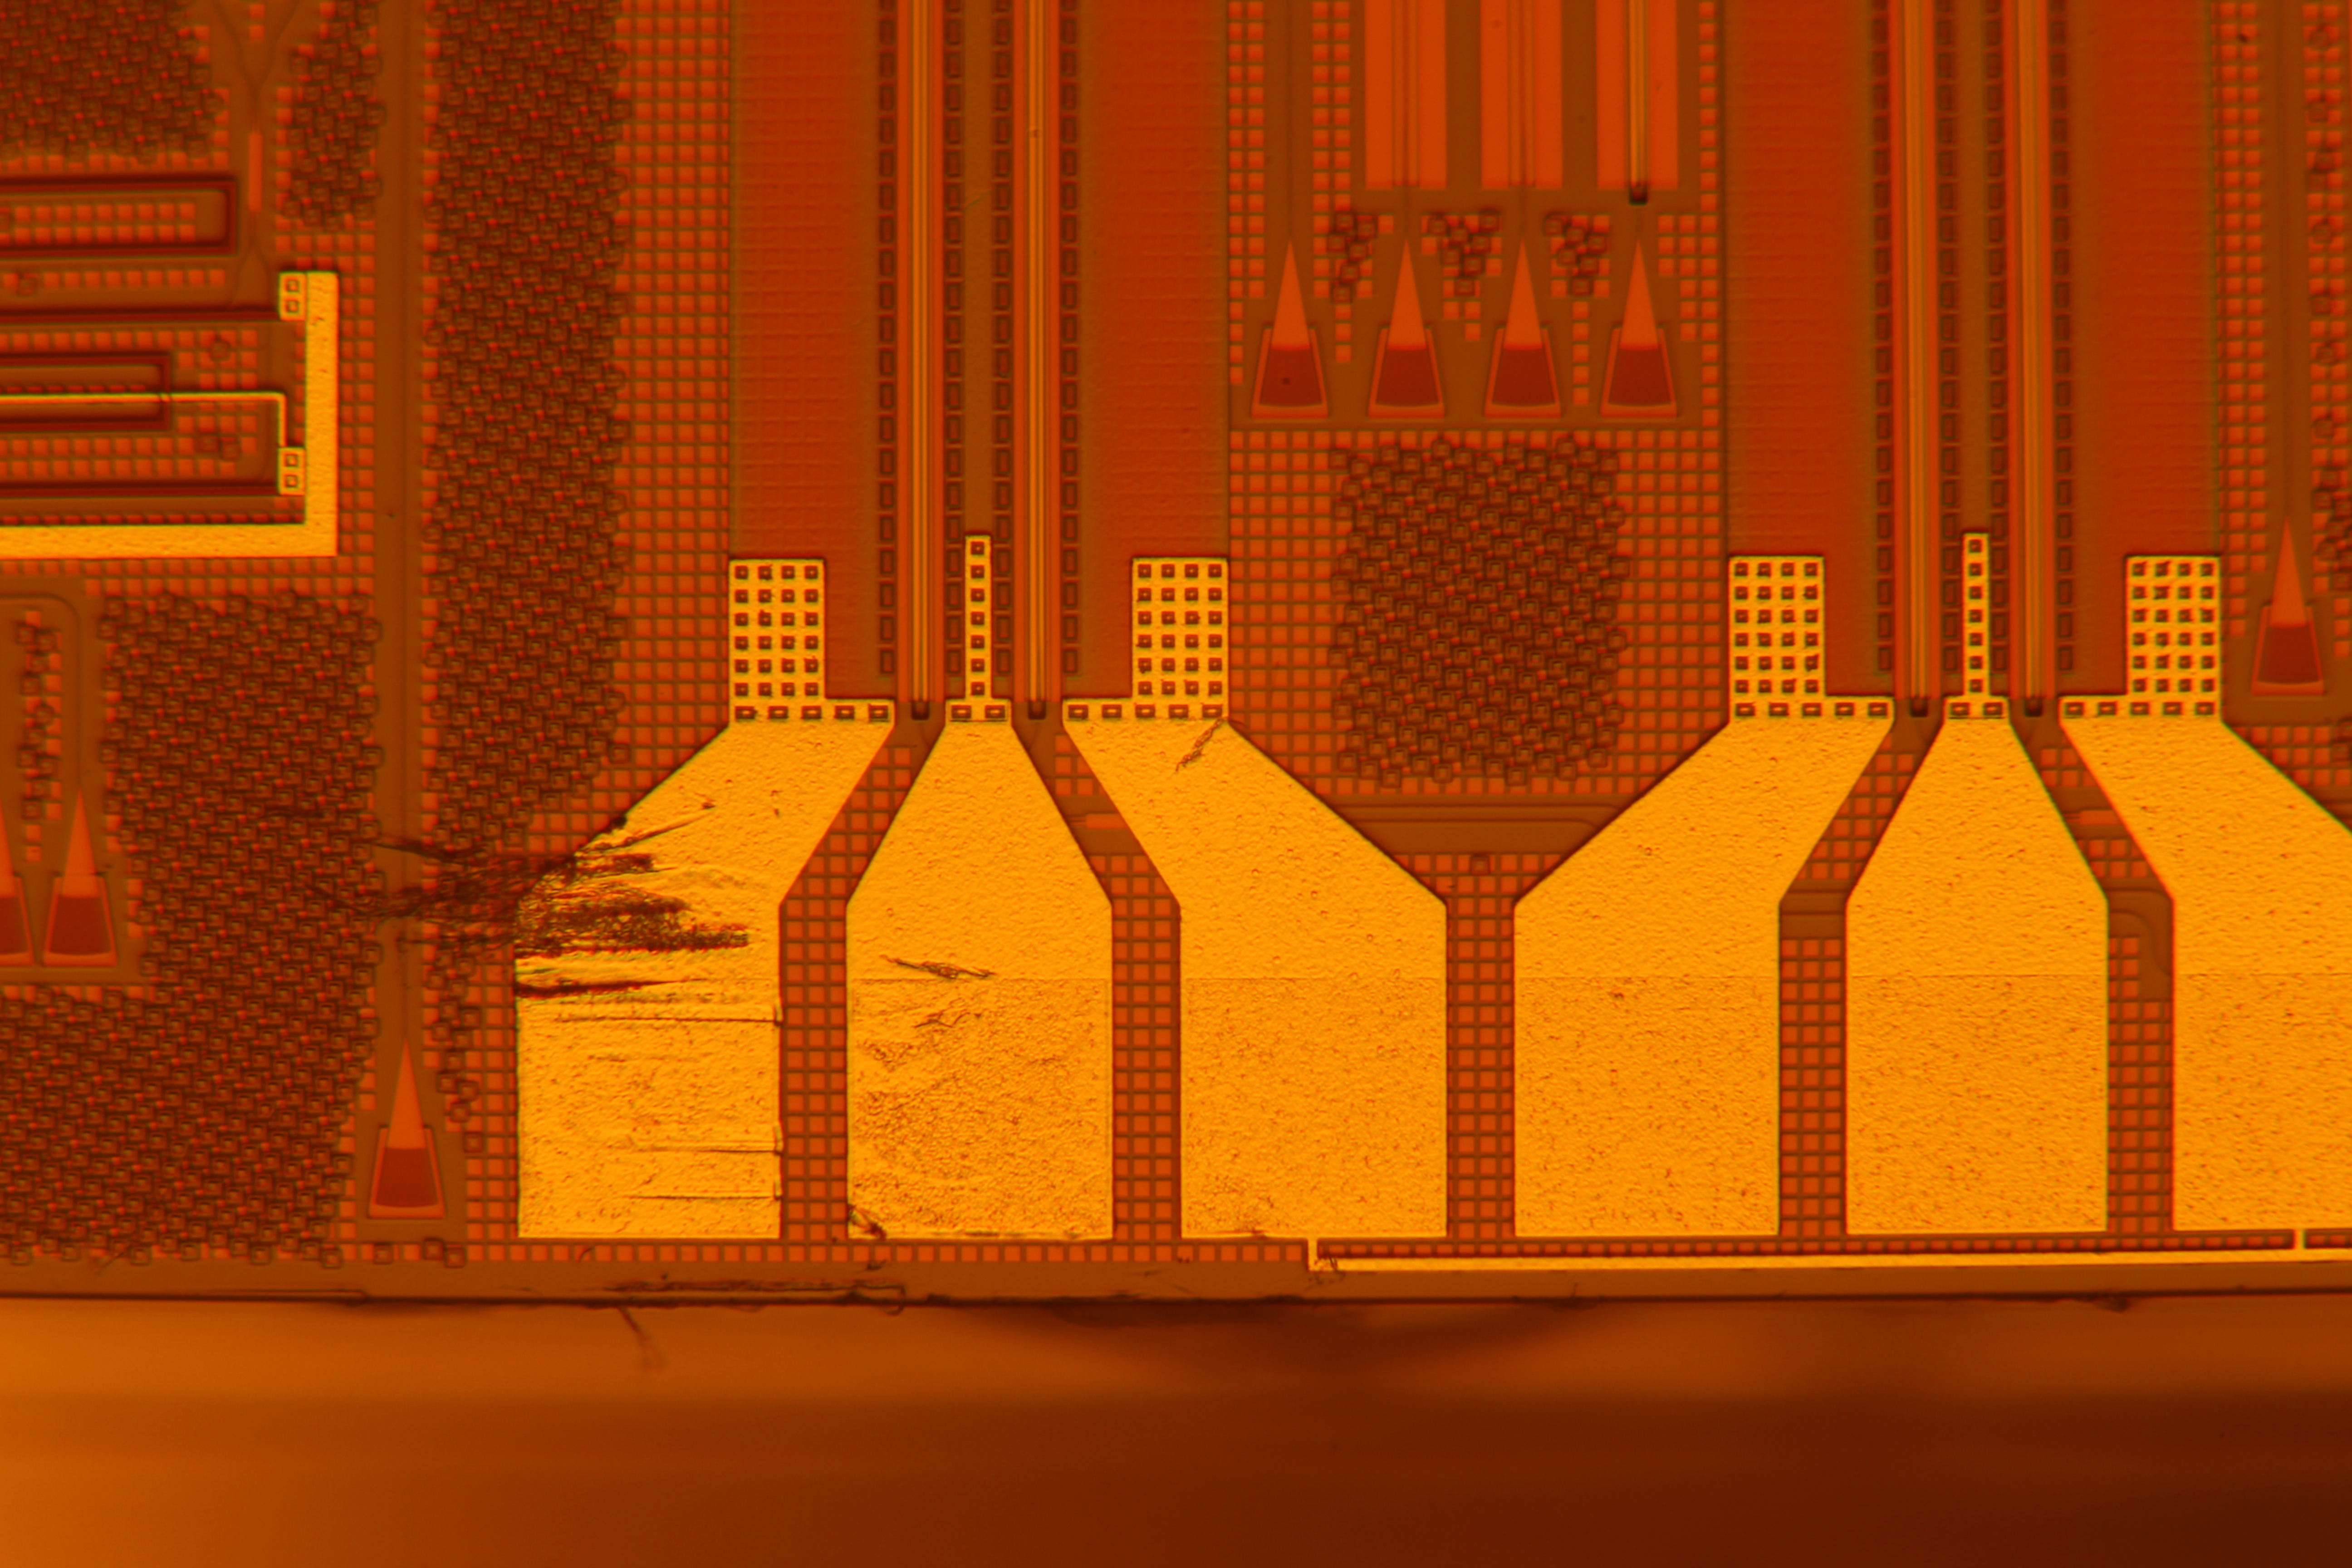
\includegraphics[width=0.42\textwidth]{lab/mcm01-02}} \\
%\subfloat[Large bend radius]{{\label{figmcm1_AS3}}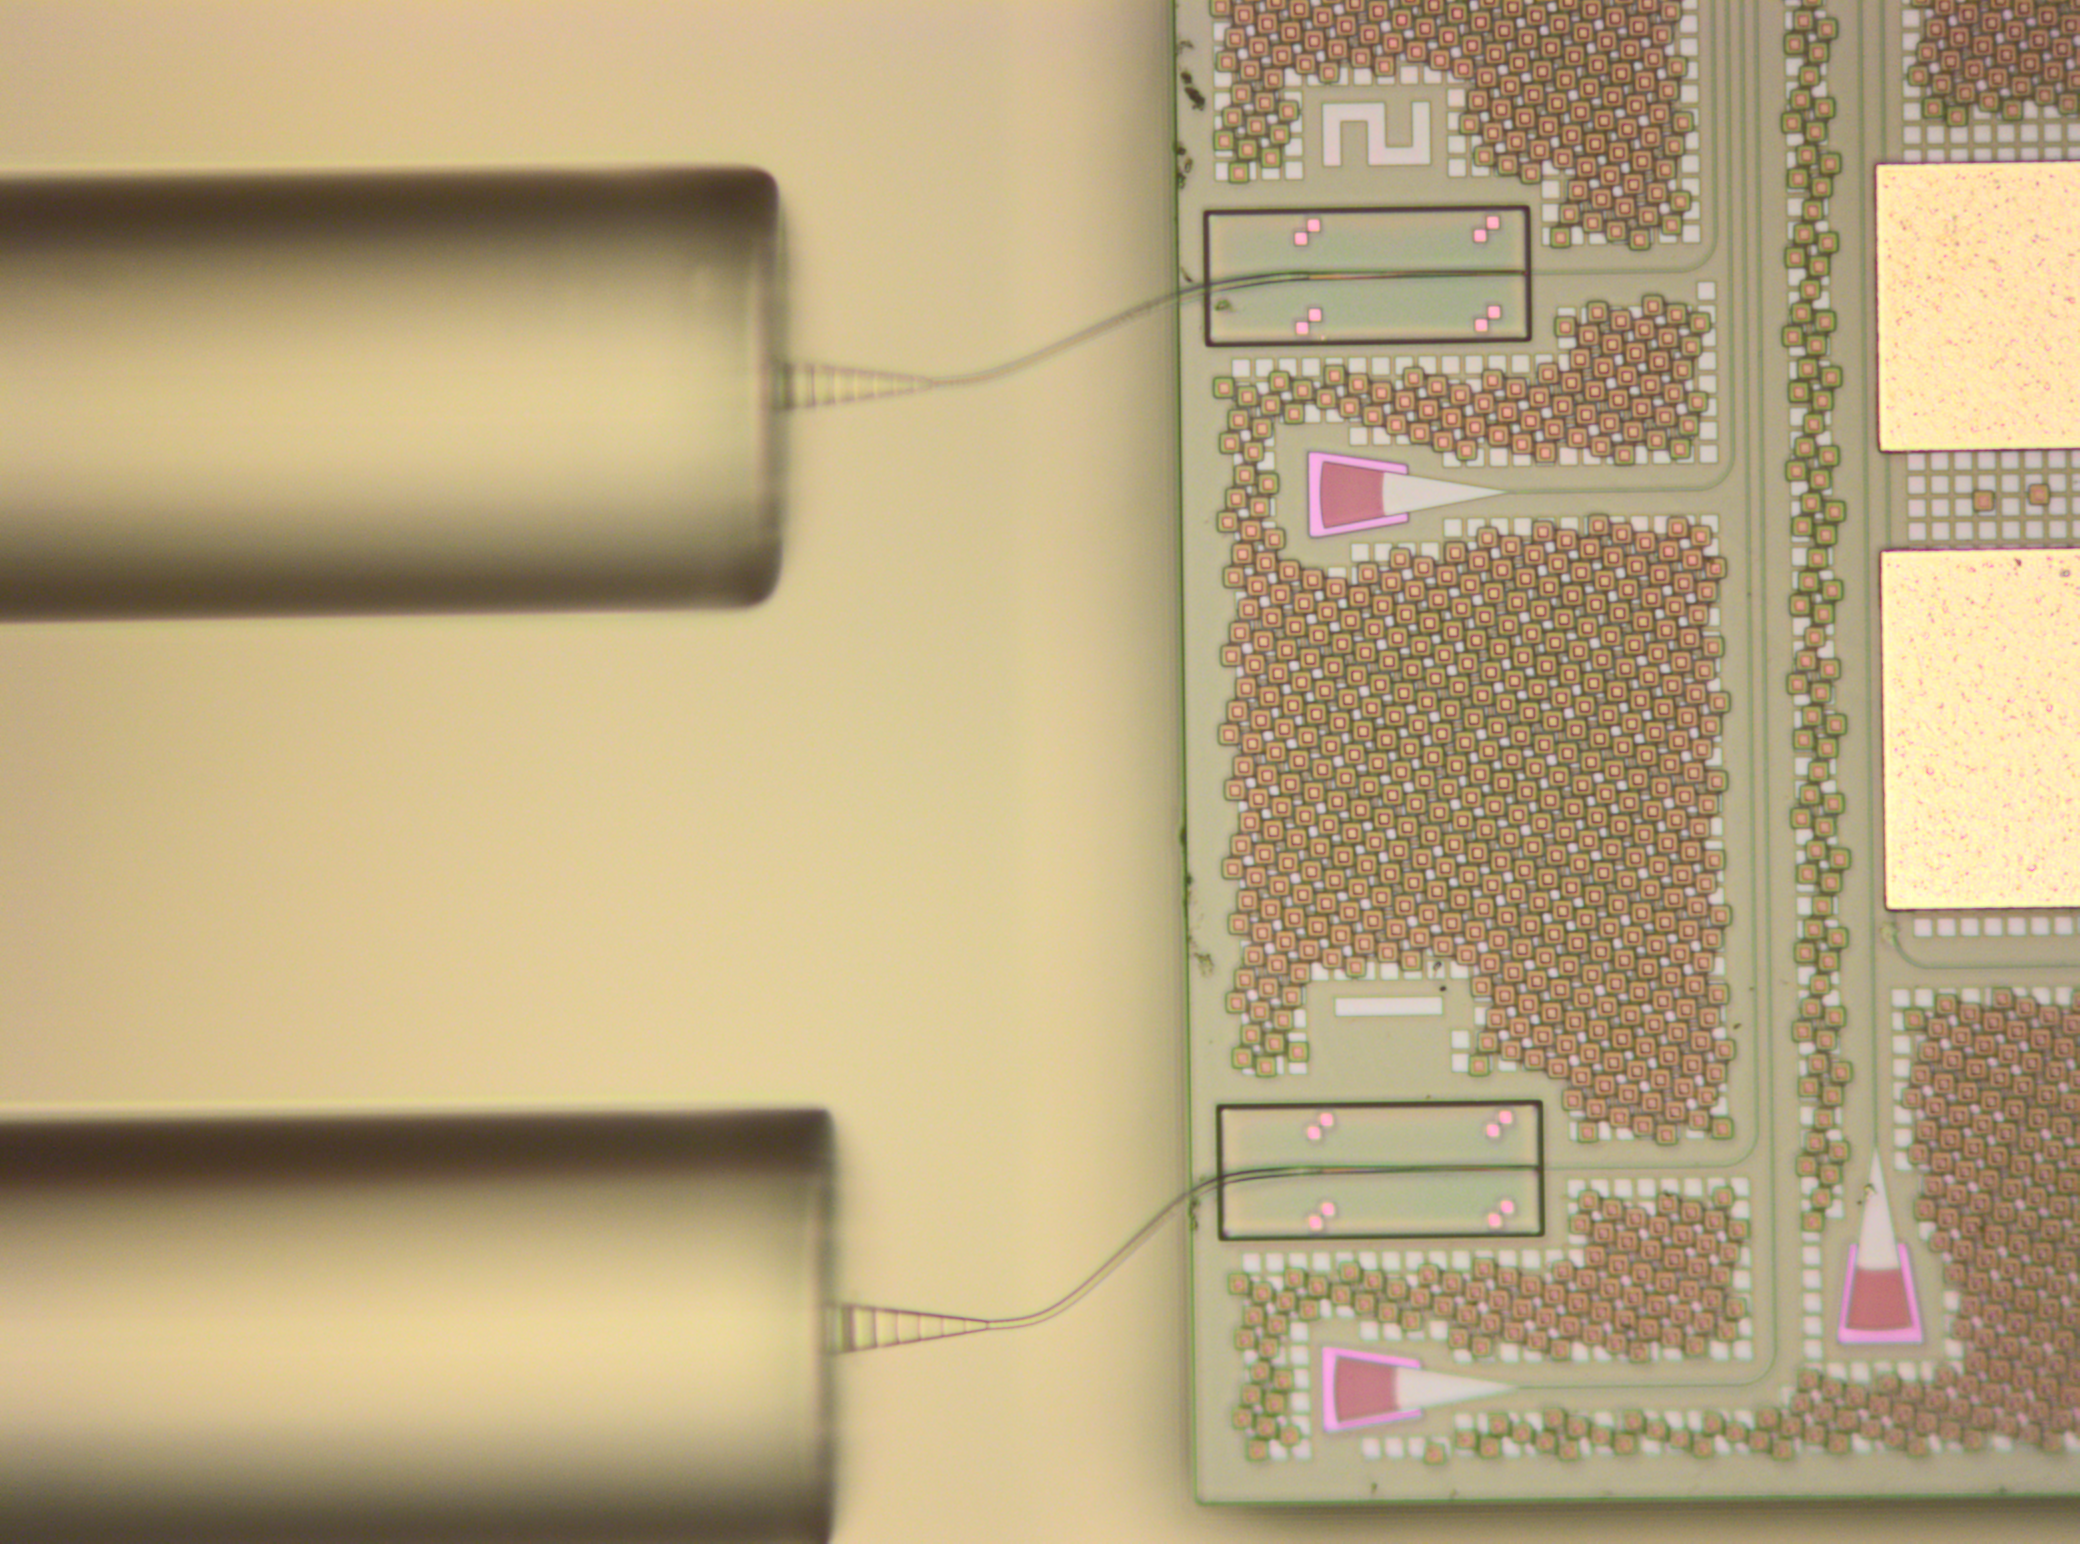
\includegraphics[width=0.42\textwidth]{lab/mcm01-03}} &
%\subfloat[Misaligned PWB]{{\label{fig:mcm1_AS4}}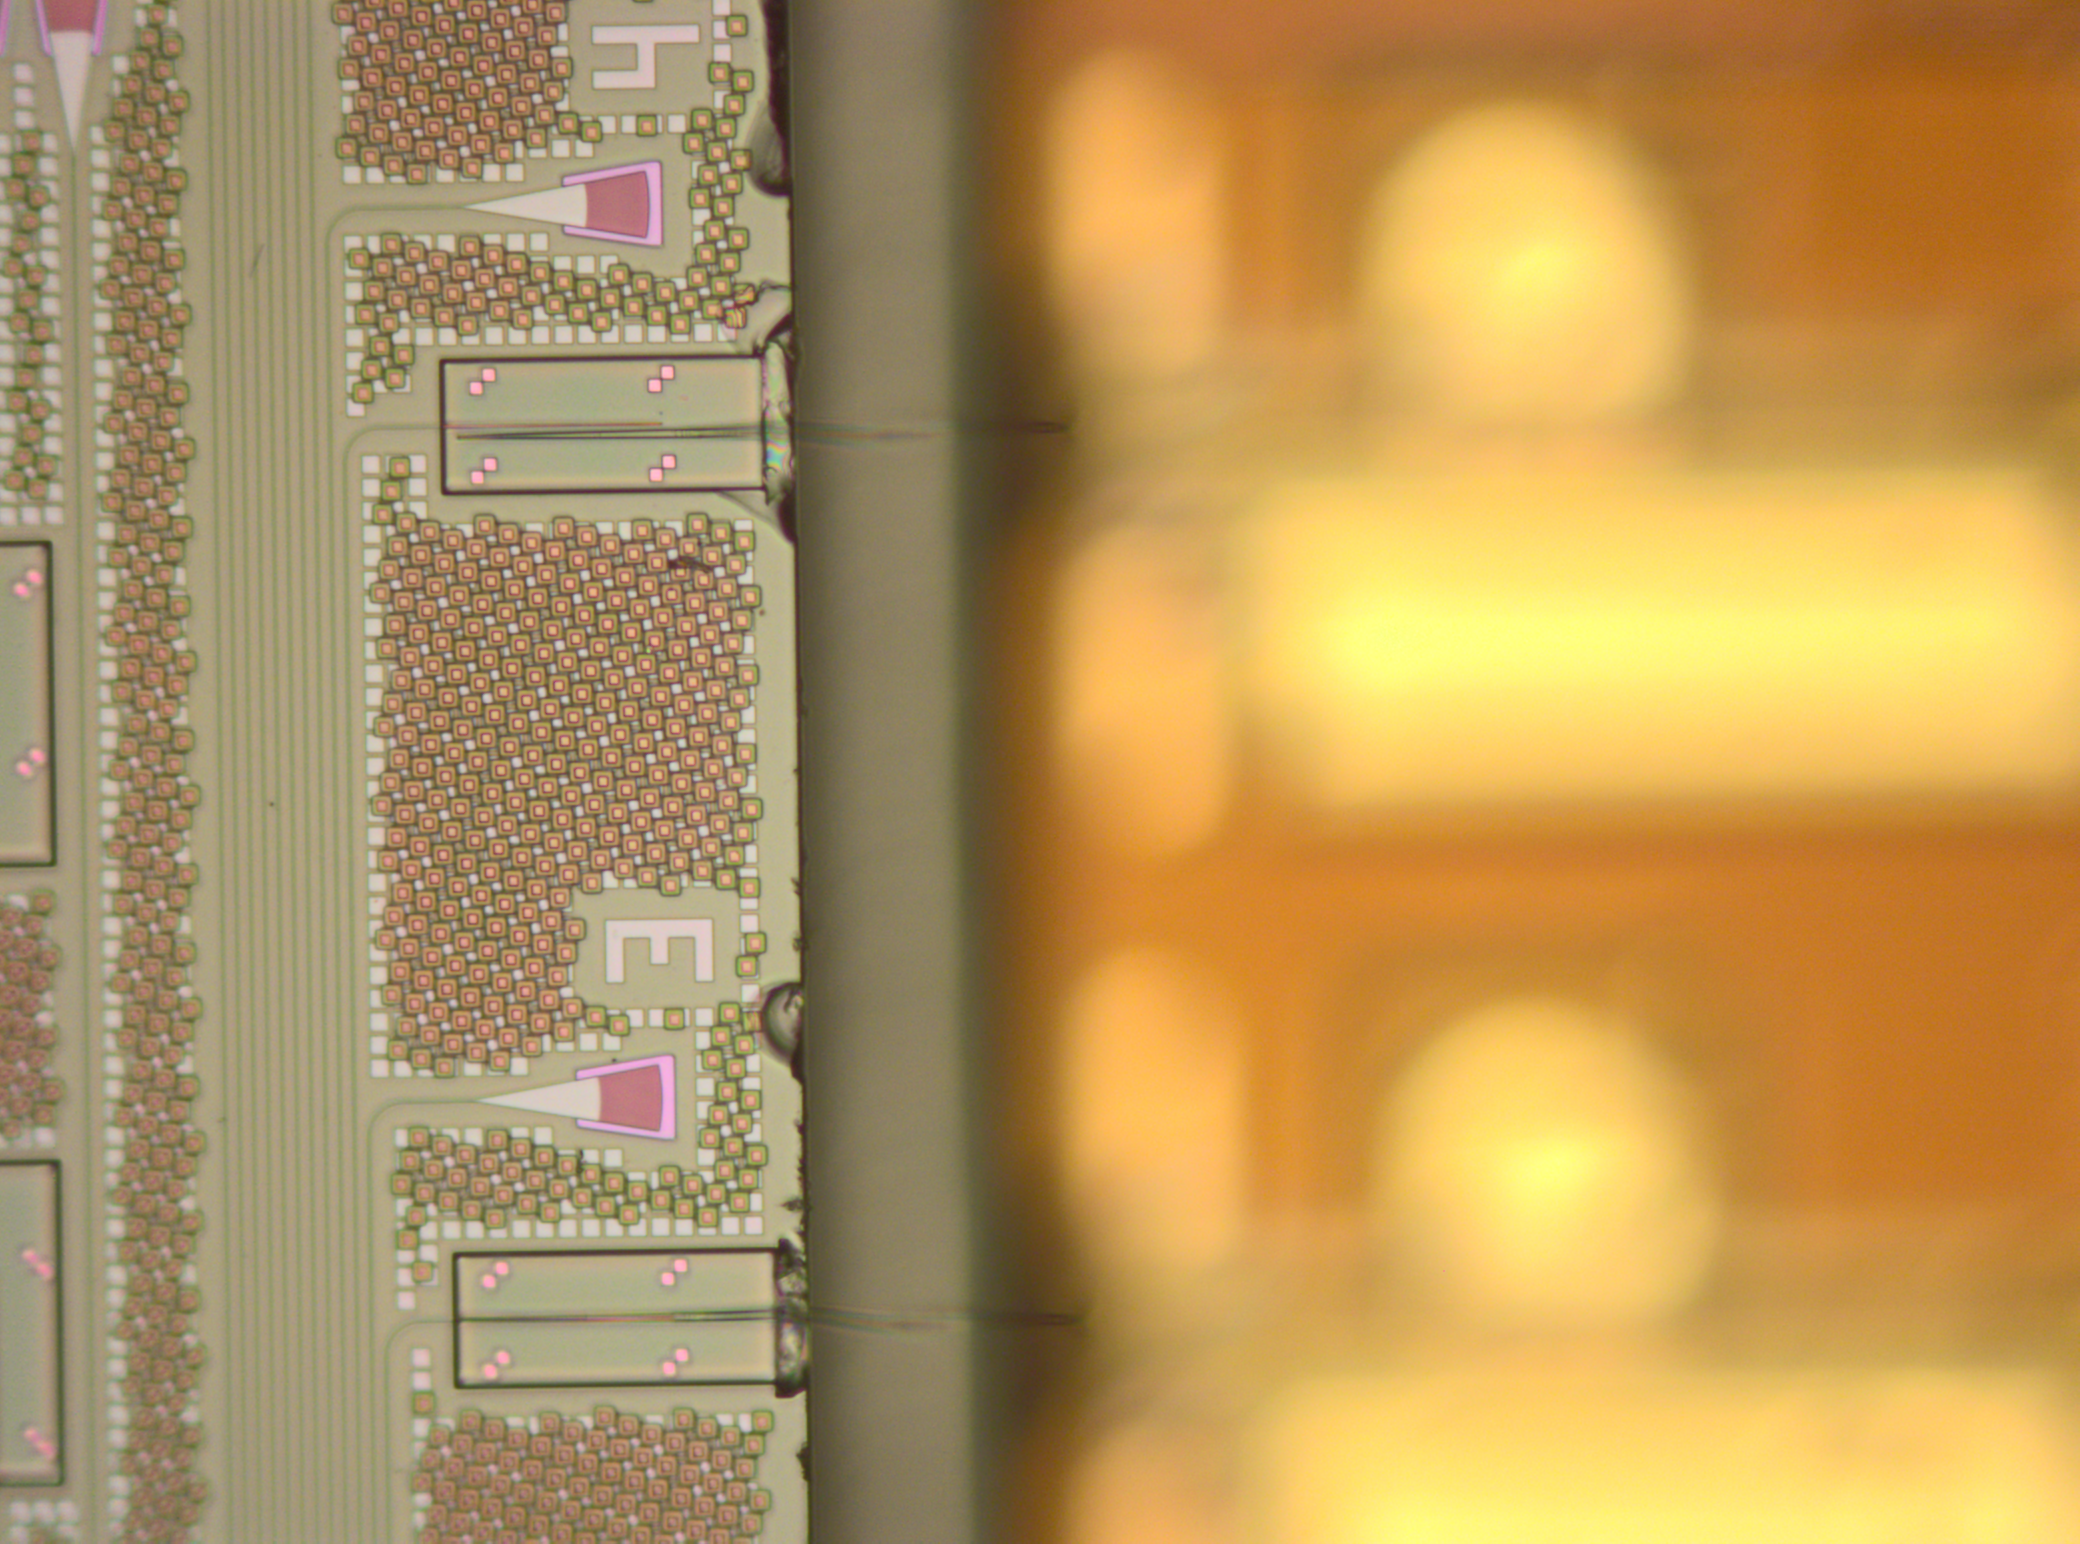
\includegraphics[width=0.42\textwidth]{lab/mcm01-05}} 
%\end{tabular}
%\caption{MCM fabrication defects.}
%\label{fig:MCM1_AS}
%\end{figure}

%The first multi-chip module (MCM) was developed focusing on full optical paths, starting from the HCSEL and reaching the output single mode fiber, with small or undetectable (by immediate visual inspection) issues with the devices. The first issues found on the devices were broken tapers; dirt in the ports (figure \ref{fig:MCM1_AS1}); and scratches due to measurements or device handling (figure \ref{fig:MCM1_AS2}). During the PWB writing process, other unexpected errors occured, such as misalignments during the writing process and miscalculations of output port location (figure \ref{fig:MCM1_AS3} and \ref{fig:MCM1_AS4}). This was only found in the first MCM. Subsequent MCMs were visually inspected to avoid using SOH chips with noticeable damage in the tapers or close to the ports that could potentially hinder the writing of PWBs. 

%% ---------------------
%% | / Example content |
%% ---------------------

The main goal of the experimental section of this master thesis with respect to the multi-chip module is achieving homogeneous transmission across all the channels of a single device. This implies that the $V_\pi$ must also be consistent among all devices, and thus it can be considered that a single, optically-packaged transmitter is capable of transmitting data at the same rate in all its channels, and thus the aggregate data rate extrapolations is valid. The following modifications were considered in search for homogeneous transmission across all channels in a device.

\subsection{Integrated Gate-Voltage Chip Module}

Application of gate voltage was thoroughly analyzed by Alloatti in his thesis \cite{gateAlloatti12}, in order to enhance the electron and hole concentration at the semiconductor interface, and thus field enhancement inside the slot which produces a highly conductive electron accumulation layer to overcome the RC speed limitation of the slot. With the improvement of the performance by application of gate voltage of the multi-chip module, a second design featuring a layered submount as shown in figure \ref{fig:MCM2-SU}, in order to avoid electrical interference in the operation of the HCSEL, because the metallic substrate ties all the grounds of the chips to a common voltage level (i.e. ground). 

The submount differs from figure \ref{fig:MCM1-SUx} by the intermediate step of the submount between the HCSEL and the SOH chip. This provides an additional space of \SI{700}{\micro\meter} to place an intermediate dielectric layer between the HCSEL and the aluminum submount. This way, the gate voltage applied to the SOH will not interfere with the HCSEL operation, in the form of an electric field across the laser diode. The selected isolation layer is an alumina (\ce{Al2O3}) slab of \SI{633}{\micro\meter} with a \SI{3}{\micro\meter} layer of gold (\ce{Au}) on top. As noted by the work of Yoshimura \cite{AluminaYoshimura81}, the dielectric breakdown of alumina is well above the voltage levels utilized in this experiment and the dielectric constant $\epsilon_R=9.6$ is sufficient to avoid any electric field interacting with the laser chip. The rest of the setup was not modified.

\begin{figure}[!ht]
\centering
  \includegraphics[width=0.9\textwidth]{visio/MCM2-SU}
  \caption{HCSEL isolation stack-up. A three-step aluminum mount is designed in-house to hold the three chips at different heights. An alumina submount with a thin gold layer is used as for the HCSEL submount. The SOH still lies on top of the aluminum mount, while the fibers are placed at the same location as previously.}
  \label{fig:MCM2-SU}
\end{figure}

\begin{table}[]
\centering
\begin{tabular}{@{}rrrrrrrrr@{}}
\toprule
Device                        & \multicolumn{1}{c}{1} & \multicolumn{1}{c}{2} & \multicolumn{1}{c}{3} & \multicolumn{1}{c}{4} & \multicolumn{1}{c}{5} & \multicolumn{1}{c}{6} & \multicolumn{1}{c}{7} & \multicolumn{1}{c}{8} \\ \midrule
Transmission {[}dBm{]}       & -22.8                  & -22.3                  & -23.0                  & -17.6                  & -44.8                  & -28.2                  & -32.9                  & -34.8                  \\
V$_\pi \cdot L$ {[}V$\cdot$mm{]} & 1.53                  & 1.64                  & 1.96                  & 1.47                  & 1.93                  & 1.40                  & 1.98                  & 1.46                  \\ \bottomrule
\end{tabular}
\caption{Transmission and $V_\pi \cdot L$ of MCM with HCSEL mounted on alumina submount summary.}
\label{tab:MCM2_sum}
\end{table}

Table \ref{tab:MCM2_sum} shows the most important figures obtained from the HCSEL isolation characterization. At first glance, there is an increase of V$_\pi$ and a very steep overall increase of the insertion loss, leading to suspicion of a process-related variations. Additionally, the HCSEL was observed to have worst parameters when in a non-metallic submount, effects which were briefly investigated in the form of the thermal roll-off observed in several HCSEL devices.
%The samples were analyzed and it was observed that there was a very visible contamination in the samples, depicted in figure \ref{fig:MCM2_contamination}. The particles were not suspected to be metallic since no electrical shorts were detected during the characterization, but the possible presence of sub-wavelength particles and air bubbles inside the slot were suspected as the main cause of the high insertion loss of the chips.

%\begin{figure}[!ht]
%\centering
%  \includegraphics[width=0.9\textwidth]{lab/mcm2_contamination_2}
%  \caption{EO polymer contamination. Demo 1 shows the initial microscope images taken in the lab, with a visibly homogeneous polymer on top of the slots. Demo 2 shows a device where there are black spots in the polymer, suspected to also contain sub-wavelength particles that deposit inside the slot and cause higher losses in the slot.}
%  \label{fig:MCM2_contamination}
%\end{figure}

%\subsubsection{Laser Threshold Current-Temperature Dependence}
%\label{sec:Evaluation:lasertemp}

%For one demonstrator, the spacer substrate submount used for the laser chip was substituted from a \SI{500}{\micro\meter} copper (\ce{Cu}) slab to a \SI{600}{\micro\meter} alumina (aluminum oxide, \ce{Al2O3}) substrate. 

The thermal conductivity of \ce{Al2O3} is 18,25 and \SI{35}{\watt/\meter\kelvin}, depending on its composition (94\%,96\% and 99.5\%, respectively). The thermal conductivity of \ce{Cu} is \SI{385}{\watt/\meter\kelvin}, according to \cite{TempYoung92}. The common carrier substrate is made of aluminum (\ce{Al}) with a thermal conductivity of \SI{205}{\watt/\meter\kelvin}. The thermal conductivity difference between alumina and copper is almost tenfold. Three very important changes to the operation conditions of the laser under a change of the submount substrate: %When analyzed as a heat sink, the heat flow can be modeled with static thermal conduction equation (why?!?!?!?!?!?!?!?!?):
%Figure \ref{fig:MCM12_LI} shows the LI curves of the operational laser chips plotted with MATLAB. The graph shows t

%\begin{align}
%k \nabla^2 T + Q = 0
%\end{align}

%Where $k$ is thermal conductivity  and $Q$ is the power density of heat. The heat sink is assumed to be a thermal reservoir at the %surface and heat extraction by air negligible, $\nabla T=0$. With thermal power density $q$ defined as:

%\begin{align}
%q = -k \nabla T
%\end{align}

%And the power density of heat can be considered constant due to the size difference of the laser chip and the heat sink. This can be easily solved by FEM. (Do the FEM) The analysis shows that higher thermal conductivity reduces temperature, but it would be expected to have an increased temperature in the laser surface, and thus a change of the operating current. 


\begin{itemize}
\item Increase of the mean threshold current of each chip of \SI{2}{\milli\ampere}
\item Decrease of the mean slope efficiency of \SI{0.18}{\milli\watt/\milli\ampere}
\item Decrease of the mean light output power of \SI{1.48}{\milli\watt} or \SI{1.7}{\decibel} attenuation
\end{itemize}

The performance decrease was due to the increase of temperature of the laser diode chip (and thus increased junction heating) due to reduced thermal conductivity of the heat sink\footnote{Thermal rollover is due to the positive feedback loop between increasing laser core temperature and threshold current density due to thermal back-filling; and Stark shift in the conduction band structure decreasing the optical dipole matrix element leading to reduced internal quantum efficiency \cite{HowardLDTher08}.}. %The thermal rollover is only observed in two lasers of MCM1 and a more consistent overall behavior in the HCSELs of MCM2. This results must be taken, nonetheless, as a naive intuition, since there was no specific thermal control implemented in the experiment, although the testing conditions and setup was relatively unchanged (i.e. no external factors were abruptly changed such as setup location and configuration, room temperature, testing time, etc.) between experiments.


%\begin{figure}[!ht]
%\centering
% \includegraphics[width=0.8\textwidth]{figs/PI_laserA4144_ith_iop_demo001-2}
%  \caption{MCM demo laser chip LI curves.}
%  \label{fig:MCM12_LI}
%\end{figure}


In the literature, the threshold current of \ce{InP} laser diodes have been analyzed for temperature dependence by Ishikawa \cite{IshikawaTempLD91}, more rigorously for \ce{GaAs} quantum well laser diodes by Menzel \cite{MenzelTempLD95} and in a simplified approximation from Nakwaski \cite{NakwaskiTempLD83}, there is no specific research that directly compares the thermal resistance of alumina and copper. %Nonetheless, a model proposed by Zhao \cite{ZhaoTempLD06} can be used for solving a simple 2D model that would provide a good approximation of the best structure for improving the thermal performance. s 

%The thermal resistance relates the dimensions of a heatsink with its thermal conductivity. For alumina:

%\begin{align}
%R_{th} = \frac{L}{k} = \frac{\SI{18.25}{\watt/\meter\kelvin}}{}
%\end{align}


%http://ieeexplore.ieee.org/stamp/stamp.jsp?arnumber=4098422

%To do:
%\begin{itemize} 
%\item Discussion of electrically-isolated current source*
%\item Discussion of HF Dip
%\item Discussion of air exposure and improvement of successful device transmission yield
%\end{itemize}
%\subsection{Process modification}

\begin{figure}[!ht]
\centering
  \includegraphics[width=0.9\textwidth]{visio/MCM3-SU}
  \caption{Gate voltage investigation setup for HCSEL changes in-operation effects. An electrically isolated current source is used to power the HCSEL and a high voltage source is used to apply gate voltage to the ground plane of the MCM.}
  \label{fig:mcm3-su}
\end{figure}

Further experimental setups were used in order to find if the electrical isolation of the HCSEL is necessary. The setup is shown in figure \ref{fig:mcm3-su}, where the current source LDX-3207 with an isolated output is used to inject current to the HCSEL chip, while a high voltage source applies voltage to the reference plane (i.e. the aluminum mount) of the MCM. No significant threshold current, operation power or spectral shift is observed in the HCSEL after application of gate voltage for 1, 3 and 5 minutes. Thus, the application of gate voltage was deemed safe for operating HCSELs for the following experiments, and electrical isolation of the HCSEL is no longer required.

%\subsection{Transmission Homogenization}
%A new module was developed in order to correct the bad transmission found earlier.
%The full process is repeated with successful writing on all devices, from pre-characterization to poling. The devices are tested in the transmission setup, using a simple GC-MZM-GC setup. The results are summarized in table \ref{tab:MCM3_sum}. %Device 7 had a transmission below detection threshold ($P_\text{launch}<\SI{-90}{\decibel}$) so no figure was obtained. Devices 6 and 8, as pointed out already, are combined ports so a free spectral range behavior can be observed. 

% Please add the following required packages to your document preamble:
% \usepackage{booktabs}
%\begin{table}[]
%\centering
%\caption{My caption}
%\label{my-label}
%\begin{tabular}{@{}rcccccccc@{}}
%\toprule
%Device                  & 1                        & 2                        & 3                        & 4                        & 5                        & 6                        & 7                        & 8                        \\ \midrule
%Insertion Loss {[}dB{]} & \multicolumn{1}{r}{29.2} & \multicolumn{1}{r}{73.4} & \multicolumn{1}{r}{41.2} & \multicolumn{1}{r}{10.7} & \multicolumn{1}{r}{20.2} & \multicolumn{1}{r}{51.7} & \multicolumn{1}{r}{$>90$} & \multicolumn{1}{r}{10.26}
%\end{tabular}
%\caption{MCM3 Summary}
%\label{tab:MCM3_sum}
%\end{table}

%\begin{figure}[!ht]
%\centering
%  \includegraphics[width=0.9\textwidth]{figs/MCM3/MZM_Transmission_demo003}
%  \caption{MCM3 Transmission.}
%  \label{fig:MCM3_TX}
%\end{figure}

%One possible explanation for the poor performance is having the devices unproperly poled: As mentioned in the theoretical framework section \ref{{sec:thbkgd:poltechs}}, if the electro-optic material is not poled, the instrinsic anisotropy of the polymer reduces charge mobility in the polymer, and thus the interaction of the RF and the optical field is severly reduced, or in the worst case scenario, neglible. A re-poling of the EO polymer was made to corroborate the effect of bad poling. Devices 2 and 3 showed transmission below threshold so no curve was recorded, while devices 1 and 4 showed no specific improvement, with the appearance of new transmission dips but improvement in other wavelengths. The process   %This lead to the assumpion that there is a  in the devices, such as sub-wavelength particles that lead to scattering, and thus requiring a change in the processing scheme.


%\begin{figure}[!ht]
%\centering
%  \includegraphics[width=0.9\textwidth]{figs/MCM3/MZM_Transmission_PrePostPoling_demo003}
%  \caption{MCM3 Re-poling (pre-poling and post-poling shown above).}
%  \label{fig:MCM3_TX_repol}
%\end{figure}

In order to modify the processing scheme, additional investigation was done on the HCSEL portion, since avoiding air exposure after HF dip is of vital importance, when the SOH chip has its PMMA overcoating and thin \ce{SiO2} removed, and thus possibly exposing the slot to external contamination. A HCSEL sample chip was then fully processed as if mounted for a multi-chip module (i.e. pre-characterization, IP dip exposition, PGMEA/isopropanol solvent bath and critical point drying), and then dipped in HF, to detect any possible changes in the electrical or optical behavior of the chip. The HCSEL was characterized in light power output and spectrum, and no significant changes were observed in its wavelength peaks or operation power ($\Delta\bar{f}=\SI{0.1}{\nano\meter}$ and $\bar{\Delta P_{op}}=\SI{0.45}{\milli\watt}$, respectively). The measurements were not done with thermal stabilization. Only minor aesthetic changes were observed in the HCSEL chip, such as the faded color coating and removal of small particles on the chip surface.

% \begin{figure}[!ht]
%\centering
%\begin{tabular}{cc}
%\subfloat[Microscope Image]{\includegraphics[width=0.40\textwidth,valign=m]{lab/HF_dip2}\label{fig:HF1}} %&
%\subfloat[Spectral Shift]{\includegraphics[width=0.5\textwidth,valign=m]{figs/HF_dip_spectralshift}\label{fig:HF2}} \\
%\end{tabular}
%\caption{HF dip effects on HCSEL. Color fading of the HCSEL coating can be observed after dipping. %Figure \ref{fig:HF2} shows the spectral shift before (red-yellow) and after (blue) dipping.
%}
%\label{fig:HFdips}
%\end{figure}

\begin{figure}[!ht]
\centering
  \includegraphics[width=0.8\textwidth]{lab/HF_dip}
  \caption{HF dip effects on HCSEL. Color fading of the HCSEL coating can be observed after dipping.}
  \label{fig:HFdips}
\end{figure}

%\begin{figure}[!ht]
%\centering
%  \includegraphics[width=0.8\textwidth]{figs/HF_dip_spectralshift}
%  \caption{HCSEL microscope view before and after HF dip.}
%  \label{fig:HF_Dip_specshift}
%\end{figure}



%\begin{itemize}
%\item Results from Demo2 (bad transmission)
%\item Results from Demo3 (HF dip, repoling, )
%\item Results from Demo4 (Characterization, results obtained)
%\item Results from Demo5 (Characterization, working still on 02.05.2017)
%\end{itemize}

%Refractive index InP 
%@1.55µm n = 3.1649 dn/dλ = -0.11135 µm-1 ng = 3.3375 GVD = 1739.6 fs2/mm D = -1363.9 ps/(nm km)
%Pettit and Turner 1965 


% Please add the following required packages to your document preamble:
% \usepackage{booktabs}
%\begin{table}[]
%\centering
%\begin{tabular}{@{}lllllllllll@{}}
%\toprule
%$\Delta \lambda$ {[}nm{]} & \multicolumn{10}{c}{Current {[}mA{]}}                                         \\ \midrule
%Device                    & 10    & 20    & 30    & 40    & 50    & 60    & 70    & 80    & 90    & 100   \\
%1                         & 0,563 & 0,155 & 0,091 & 0,012 & 0,137 & 0,293 & 0,46  & 0,71  & 0,986 & 1,293 \\
%2                         & 0,014 & 0,044 & 0,038 & 0,046 & 0,039 & 0,053 & 0,062 & 0,079 & 0,13  & 0,121 \\
%3                         & 0,042 & 0,037 & 0,031 & 0,01  & 0,022 & 0,018 & 0,052 & 0,074 & 0,119 & 0,106 \\
%4                         & 0,007 & 0,032 & 0,021 & 0,011 & 0,003 & 0,034 & 0,081 & 0,102 & 0,109 & 0,144 \\
%5                         & 0,008 & 0,008 & 0,019 & 0,028 & 0,031 & 0,012 & 0,02  & 0,013 & 0,042 & 0,075 \\
%6                         & 0,001 & 0,001 & 0,003 & 0,01  & 0,013 & 0,029 & 0,085 & 0,111 & 0,136 & 0,171 \\
%7                         & 0,028 & 0,028 & 0,035 & 0,04  & 0,037 & 0,04  & 0,031 & 0,028 & 0,016 & 0,006 \\
%8                         & 0,039 & 0,048 & 0,072 & 0,085 & 0,118 & 0,138 & 0,146 & 0,15  & 0,165 & 0,191 \\ \bottomrule
%\end{tabular}
%\caption{Wavelength shift before and after HF dip per current step in HCSEL.}
%\label{tab:lambdashift_HFdip}
%\end{table}

\subsection{Modified Process Flow and Results}

\begin{figure}[!ht]
\centering
  \includegraphics[width=0.9\textwidth]{visio/final_process}
  \caption{Final process flow for multi-chip module (MCM) production. The key changes rely on complete MCM mounting and further process the whole device by dipping in acetone and HF for PMMA \ce{SiO2} dissolution, respectively, and thus avoiding slot exposure to the environment.}
  \label{fig:fproc}
\end{figure}

The final process flow developed in this master thesis featuring consistent $V_\pi$ and transmission is shown in figure \ref{fig:fproc}. The key improvements done to the process are the following:

\begin{enumerate}
\item \textbf{HCSEL process modification:} With the knowledge that there is no effect in the HCSEL in the HF dip chemical treatment, the possibility to process the whole module through the removal of PMMA and native silicon oxide was deemed reliable. 
\item \textbf{SOH mounting process modification:} This meant that the SOH device would also have to be reliable during the mechanical mounting of the HCSEL. The thermal curing of the epoxy used can be reduced in temperature at the cost of increasing the exposure time. This is critical to avoid the glass transition temperature of PMMA, sitting between \SI{85}{\celsius} and \SI{165}{\celsius}, so the temperature is chosen below the lowest limit to avoid hardening of PMMA which can change the dissolving dynamics during the following processes.
\item \textbf{PWB development modification:} The time in which the module sits in PGMEA and isopropanol is increased to ensure there are no traces of IP-dip inside the slot after the PWB writing. This was taken as a cautionary measure, considering the previously observed correlation between the exposure of the slot and the final EO polymer deposition.
\end{enumerate}

\begin{figure}[!ht]
\centering
  \includegraphics[width=0.85\textwidth]{figs/MCM4/MCM4_IL_measured_demo004}
  \caption{Improved process flow MCM transmission function. Devices 1 and 8 are not accesible in IQ configuration. The grating coupler transmission function is still visible.}
  \label{fig:MCM4_TX}
\end{figure}

\begin{table}[]
\centering
\begin{tabular}{@{}rrrrrrrrr@{}}
\toprule
Device                        & \multicolumn{1}{c}{1} & \multicolumn{1}{c}{2} & \multicolumn{1}{c}{3} & \multicolumn{1}{c}{4} & \multicolumn{1}{c}{5} & \multicolumn{1}{c}{6} & \multicolumn{1}{c}{7} & \multicolumn{1}{c}{8} \\ \midrule
V$_\pi \cdot L$ {[}V$\cdot$mm{]} & N/A                  & 1.36                  & 1.37                 & 1.3                  & 1.36                  & 1.36                  & 1.32                  & N/A                  \\ \bottomrule
\end{tabular}
\caption{$V_\pi \cdot L$ measurement of improved process flow MCM. Devices 1 and 8 are not accessible in the IQ configuration.}
\label{tab:MCM2_sum}
\end{table}

The above changes were implemented in the final demonstrator, a \SI{1}{\milli\meter} IQ modulator. The module was processed in a way that avoided air exposure of the slots until the EO polymer deposition, meaning that between the HF dip and the PWB writing, the chip was sealed and transported between clean rooms without exposition to light or air. The transmission of 6 MZM is plotted in figure \ref{fig:MCM4_TX}, and it shows a very consistent transfer function across all modulators. The transmission of the grating coupler can still be observed, which was not recorded at the moment of initial characterization due to time constraints. The former results  that avoiding air exposure of the slots gives a homogeneous transmission across the device due to minimal external agents introduced to the slot.



\subsection{Thermal Roll-off Analysis}
Thermal roll-off was observed in few HCSEL units with no specific correlation to external damage due to handling, such as scratching of the anode or cathode pads; damage of the ridge waveguide due to scratching; or general external structural characteristics of the HCSEL. Buried heterostructure laser diodes (such as the HCSEL used here), exhibit gradual performance degradation due to possible defects created during the mesa etch and regrowth of the sidewall of the active and cladding layer \cite{SwinglerThermal14}. Thus, the  morphology of the HCSEL layers is of vital importance to understand the roll-off phenomenon.

\begin{figure}[!ht]
\centering
\begin{tabular}{cc}
\subfloat[LI Curve]{\includegraphics[width=0.5\textwidth,valign=m]{figs/MCM4/LI_laserA41_ith_iop_demo004}\label{fig:LI_TR_2}} &
\subfloat[Spectrum]{\includegraphics[width=0.5\textwidth,valign=m]{figs/MCM4/SPK/HCSEL1_Spectrum_demo004_PRE}\label{fig:Df_SPK_2}}  \\
\end{tabular}
\caption{HCSEL Roll-off behavior. A HCSEL with increasingly prominent thermal roll-off is pre-characterized in light-current and spectral configurations.}
\label{fig:HCSELTR_rolloff}
\end{figure}

A quantitative but indirect approach to observe such behavior is depicted in the following. The spectrum of HCSEL arrays were recorded during the pre-characterization of the devices, paying special attention to those chips which show thermal roll-off. 

\begin{figure}[!ht]
\centering
\begin{tabular}{cc}

\subfloat[Wavelength shift]{\includegraphics[width=0.5\textwidth,valign=m]{figs/MCM3/HF_Dip/SPK/HCSEL8_Spectrum_demo003_wlshiftPREPROC}\label{fig:Df_SPK}} &
\subfloat[Wavelength peaks]{\includegraphics[width=0.5\textwidth,valign=m]{figs/MCM3/HF_Dip/SPK/HCSEL8_Spectrum_demo003_wlshiftPREPROC_peaks1}\label{fig:LI_TR}}  \\
\end{tabular}
\caption{HCSEL normal condition behavior.}
\label{fig:HCSELTR_normal}
\end{figure}

In figure \ref{fig:HCSELTR_normal}, The behavior of a normally-operating HCSEL is shown. Figure \ref{fig:Df_SPK} shows the wavelength shift that occurs during a current change of $\Delta i = \SI{10}{\milli\ampere}$. In figure \ref{fig:LI_TR}, the wavelength peaks can be observed for each HCSEL array and it is also notable that the wavelength peak spacing is consistent across the devices, and thus, there is no wavelength overlap .

\begin{figure}[!ht]
\centering
\begin{tabular}{cc}
\subfloat[Wavelength shift]{\includegraphics[width=0.5\textwidth,valign=m]{figs/MCM4/SPK/HCSEL4_Spectrum_demo001_wlshiftHCSEL4_Spectrum_demo00}\label{fig:Df_SPK4}}  &
\subfloat[Wavelength peaks]{\includegraphics[width=0.5\textwidth,valign=m]{figs/MCM4/SPK/HCSEL4_Spectrum_demo001_wlshiftPREPROC_peaks1HCSEL4_Spectrum_demo00}\label{fig:Df_SPK5}}  \\
\end{tabular}
\caption{HCSEL Roll-off relative shift and peaks.}
\label{fig:HCSELTR_rolloff_peaks}
\end{figure}

In the case where a HCSEL features heavy roll-off, such as that in \ref{fig:HCSELTR_rolloff}, the LI curve shows increasingly high thermal roll-off, and the spectrum of the HCSEL that has the worst case roll-off. As expected, spectral hole burning is observed. It is however more interesting to see the relative shift and peaks in the case of heavy roll-off, as observed in figure \ref{fig:HCSELTR_rolloff_peaks}, with an increase of the slope in the relative wavelength between current steps, and a heavier red shift of the wavelength of the laser as current is increased. There is also a very noticeable overlap of the wavelength peaks, which makes the HCSEL array no longer reliable for applications such as WDM, because of the very likely overlap of wavelengths in a combined channel.

The spectral shifting of a HCSEL due to increased temperature can be correlated to the refractive index change in the buried heterostructure, through the relation \cite{BainTemp10}:

\begin{align}
 \frac{d \lambda}{d T} \propto \frac{d \tilde n}{dT}
\end{align}

And thus, as postulated previously, a slight structural change in the manufacturing of the HCSELs can thus show that a change of the thermal operation of the HCSEL, indicates a change of the refractive index inside the buried heterostructure, and thus, defects in the layer stack-up of the HCSEL. Specific structural analysis can be done with SEM pictures of the internal structure of the HCSEL, but such studies are outside of the scope of the work in the present master thesis. This provides some insights on the thermal roll-off phenomenon in HCSEL chips, which is not related to external structural issues but from the fabrication process of the device itself.
%\input{sections/content.tex}
%% LaTeX2e class for student theses
%% sections/evaluation.tex
%% 
%% Karlsruhe Institute of Technology
%% Institute for Program Structures and Data Organization
%% Chair for Software Design and Quality (SDQ)
%%
%% Dr.-Ing. Erik Burger
%% burger@kit.edu
%%
%% Version 1.2, 2016-09-20

\chapter{Data Transmission Experiments}
\label{ch:Evaluation}

The final proof-of-principle to demonstrate the functionality of a multi-chip module is the realization of a real data transmission experiment that uses the built MCM as the data source, and is received by an optical receiver that demodulates and interprets the information carried in the lightwave in a communication link. The receiver used are characterized, unamplified photodiode modules that decouple the receiver behavior from the transmitter performance, such that the latter can be assessed through the results of the data transmission experiment.
\par\medskip
In this chapter, the details of the implementations used throughout the data transmission experiments procedure are discussed and reviewed. The description of the demonstrators featuring direct detection (MZM modulator) and coherent detection (IQ modulator) are presented, including the setup used for each case and the discussion of the results obtained. All measurements were done with PWB with air as an overcladding.

%\textbf{Data transmission experiment}: The final step to corroborate the performance of the multi-chip module requires the device to be tested  transmitting sample data in order to characterize its transmission properties. The bit error probability (BER) is the most significant figure of merit, along with the external testing conditions (use of erbium-doped fiber amplifier (EDFA); use of gate voltage; use of attenuators, etc.) used to reach such quantity.

\section{Direct Detection Data Transmission Experiment}

\begin{figure}[!ht]
\centering
  \includegraphics[width=0.8\textwidth]{visio/MCM-LO_DTE}
  \caption{Initial MCM direct detection data transmission experiment. The HCSEL is powered by a precision current source set at \SI{100}{\milli\ampere}. For data injection, a pulse pattern generator (PPG) with an RF amplifier  is connected to the MZM signal probe, terminated with a \SI{50}{\ohm} external resistor. The launched light is connected through an angled connector to the photoreceiver and analyzed with a scope.}
  \label{fig:mcm-001-DTE}
\end{figure}

The components used in the direct detection data transmission experiment setup are schematically represented in figure \ref{fig:mcm-001-DTE}. A high-precision external current source is set to \SI{100}{\milli\ampere} to provide power for the HCSEL. The MZM signal terminal is impedance-matched with a \SI{50}{\ohm} termination resistor, and a programmable pattern generator (PPG) with an RF amplifier is used as a signal source to modulate the MZM, coupled to the circuit with a bias tee and an independent external voltage source. The modulated signal is sent through a single mode fiber (SMF) with an angled connector (APC) to a photodiode receiver into a scope to analyze the corresponding received signal. The eye diagram mask is shown in figure \ref{fig:MCM1}. The calculated BER is obtained as in appendix \ref{sec:appendix:calcBER}, yielding a value of \SI{2.2e-3}. %In this case, \SI{10}{\giga bit/\second}, and no EDFA or gate voltage is applied. The signal obtained is only the electrical eye diagram. 

\begin{figure}[!ht]
\centering
  \includegraphics[width=0.8\textwidth]{visio/MCM-LO_DTE_GV}
  \caption{First MCM data transmission experiment with gate voltage implemented diagram. Light is injected to the MZM through an external tunable laser source (TLS). For data injection, a pulse pattern generator is connected to an RF amplifier and a bias tee through a GSG picoprobe. The MZM is terminated with a \SI {50}{\ohm} external resistor. The outcoupled light is detected by a photoreceiver connected to a vector signal analyzer (VSA). Gate voltage (inside a dashed line) was added later in the process.}
  \label{fig:mcm-001-DTE-GV}
\end{figure}


\begin{figure}[!ht]
\centering
\begin{tabular}{cc}
\subfloat[\SI{10}{\giga bit/\second},$V_\text{gate}=\SI{0}{}$, no EDFA]{\includegraphics[width=0.45\textwidth]{caps/opt_10G_gate50V_noedfa}\label{fig:MCM1}} &
%\subfloat[E, \SI{40}{\giga bit/\second},$V_\text{gate}=\SI{50}{\volt}$, with EDFA]{\includegraphics[width=0.45\textwidth]{caps/el_40G_gate50V_edfa}\label{fig:MCM2}} \\
\subfloat[\SI{40}{\giga bit/\second},$V_\text{gate}=\SI{50}{\volt}$, with EDFA]{\includegraphics[width=0.45\textwidth]{caps/opt_40G_gate50V_edfa}\label{fig:MCM3}} %&
%\subfloat[O, \SI{10}{\giga bit/\second},$V_\text{gate}=\SI{100}{\volt}$, with EDFA]{\includegraphics[width=0.45\textwidth]{caps/opt_10G_gate50V_noedfa}\label{fig:MCM4}} 
\end{tabular}
\caption{MCM direct detection eye diagrams; Data rate for each case are noted, as well as the applied gate voltage and whether an EDFA was used for optical amplification.}
\label{fig:MCM_gateEDFA}
\end{figure}
%\begin{figure}[!ht]
%\centering
%  \includegraphics[width=0.8\textwidth]{caps/SOH_10G_E_NOG}
%  \caption{MCM eye diagram at \SI{10}{\giga bit/\second}, \SI{20}{\pico\second/div}.}
%  \label{fig:mcm-001-eye1}
%\end{figure}

%\lasnotas{which is driven to depletion, and thus no free carrier absorption occurs,  and thus a slot waveguide lying on top of an insulating layer (in the specific case of this thesis, \ce{SiO2}) will present band bending due to majority carrier accumulation. MAYBE PUT THIS SOMEWHERE ELSE}.  The MCM was tested at \SI{40}{\giga bit/\second}, but no eye was visible under the aforementioned conditions. 
In order to further push the performance of the MCM, the addition of gate voltage and the use of an erbium-doped fiber amplifier (EDFA) was suggested and added to the setup. The schematic diagram of the setup is presented in figure \ref{fig:mcm-001-DTE-GV}. As explained in appendix \ref{sec:appendix:gatevolt}, a large positive voltage is applied to the silicon (\ce{Si}) substrate to allow inversion in the metal-semiconductor-isolator boundary and thus allowing for improved carrier concentration and mobility. The setup also changes to an external laser source (ECL), since there was a suspicion of possible damage to the HCSEL due to the ground of the first demonstrator MCM being tied together (due to the metallic aluminum substrate). The launch is done through the PWB through the APC connector and an EDFA with a filter is used to amplify the optical signal and analyzed with a scope.



Figure \ref{fig:MCM_gateEDFA} shows the most prominent results of the data transmission experiment using an MZM modulator. In figure \ref{fig:MCM1} the device is tested at low transmission speeds and measuring the optical eye mask. It can be seen that the eye rise time has a smaller slew rate than the falling edge causing duty-cycle jitter. This can be phenomenologically explained by the Mach-Zender modulator being slightly unbalanced, much like its analog effect in RF electrical circuits, referred to as common mode noise \cite{DjordjevicCM10}. The effect can be translated to optical fields due to an inhomogeneous field distribution where the gate voltage is applied. The effect was reviewed in super-junction LDMOS (laterally-diffused metal-oxide semiconductors) in an SOI substrate by Wang \cite{WangGV09}, where charge imbalance in the junction requiring tuning of the charges in the semiconductor junction regions. Since the structure of the MZM also has different electric field interactions in each arm, the results observed in the work of Wang. Figure \ref{fig:MCM3} show the case for gate voltage applied, for optical detection. The results reveal a promising result towards \SI{100}{\giga bit/\second} fully-functional performance, which was not tested because of the equipment limitation (the highest achievable data rate for direct detection is \SI{40}{\giga bit/\second} with the current settings). Finally, the data transmission experiment shows that there is no inherent data rate limitation on the SOH device.   %Finally, figure \ref{fig:MCM3}, shows an increased gate voltage test, which again shows duty-cycle jitter due to rise and fall time asymmetries.
%\FloatBarrier
%\clearpage

\section{Coherent Detection Data Transmission Experiment}

\begin{figure}[!ht]
\centering
  \includegraphics[width=0.8\textwidth]{visio/MCM-LO-IQ-DTE}
  \caption{MCM IQ data transmission experiment diagram. Light is coupled to the MZM through a PWB connected to a HCSEL, and externally modulated. An arbitrary waveform generator (AWG) with at least two channels is connected via an RF amplifier and a bias tee to each branch of the IQ modulator and terminated externally with \SI{50}{\ohm} resistors. Light is outcoupled to an EDFA, an passband filter and visualized through a VSA. Gate voltage is applied externally to the submount of the chip.}
  \label{fig:mcm-005-DTE-IQ}
\end{figure}

The next data transmission experiment was done after a homogeneous $V_\pi$ and transmission were obtained through processing iterations, and an IQ modulation was chosen because it proves the performance of the SOH platform, at the expense of more difficult fine tuning and a more complex setup, which is shown schematically in figure \ref{fig:mcm-005-DTE-IQ}. The data injection scheme is now done through an arbitrary wave generator (AWG) with 4 channels, connected through a bias tee using GSG microprobes on both sides of the MCM, and terminated with \SI{50}{\ohm} resistors for each modulator. A gate voltage $V_\text{gate}=\SI{100}{\volt}$ is applied to the module for its known improvement of the chip performance. The IQ modulators feature thermal phase shifters, consisting on resistive layers in the IQ modulator that can be modified through voltage, also controlled by an external DC source up to \SI{5}{\volt}. At the fiber output, an EDFA is connected to a bandpass filter and connected to an optical modulation analyzer (OMA) for visualization of the eye diagrams.

Each arm of the IQ modulator is independently optimized for best performance, and then calibrated for jitter and skew of both arms. Thermal shifters are used to obtain the optimum pre-compensation which was post-processed and applied to achieve the best possible transmission. Finally, a Kalman filter for phase tracking was implemented to overcome the considerable phase noise of the HCSEL. Another possible limitation was due to the relatively high $V_\pi$ of the SOH modulators. Nonetheless, it is low enough that non-linearities are observed in 16QAM modulation when using RF amplifiers. Figure \ref{fig:mcm-005-DTE-res} shows the summary of the measurements, with the best achievable speed being 16QAM, 56 Gbaud featuring a bit error probability (BER) of \SI{8e-3}{} and a forward error correction (FEC) of 20\%, with a total potential transmission data rate of 716 Gbit/s.

\begin{figure}[!ht]
\centering
  \includegraphics[width=0.8\textwidth]{caps/IQ_56gb}
  \caption{MCM IQ result summary. QPSK and 16QAM modulation was used to test the performance of the IQ modulator. Speeds of 32, 46 and 56 Gbaud were used and evaluated in error vector magnitude (EVM) QPSK and bit error probability (BER) for QPSK and 16QAM. Forward error correction (FEC) was considered for 16QAM format.}
  \label{fig:mcm-005-DTE-res}
\end{figure}

%% -------------------
%% | Example content |
%% -------------------


%% LaTeX2e class for student theses
%% sections/conclusion.tex
%% 
%% Karlsruhe Institute of Technology
%% Institute for Program Structures and Data Organization
%% Chair for Software Design and Quality (SDQ)
%%
%% Dr.-Ing. Erik Burger
%% burger@kit.edu
%%
%% Version 1.2, 2016-09-20

\chapter{Summary and Outlook}
\label{ch:Conclusion}

A stable process flow for optical packaging of multi-chip modules combining SOH devices with PWB was successfully achieved in the period of development of this master thesis. An initial single-channel device was successfully fabricated with low $V_\pi$ and good transmission of the multi-chip module. The integration process was successfully tested with the first direct detection data transmission experiment using integrated PWB and SOH devices up to 40 Gbit/s, with no specific limitation on the SOH side to achieve 100 Gbit/s parallel single mode direct detection transmission. 
Through fine tuning and arrangement of the full processing methodology, it was also possible to achieve a homogeneous, consistent  transmission of SOH modulators, with a $V_\pi=\SI{1.3}{\volt\milli\meter}$ that allowed proof-of-concept of data transmission using 16QAM modulation at 56 GBaud with no refractive index-matching oil or UV glue as an overcladding.
\par \medskip
The outlook of the project towards a fully-integrated terabit multi-chip module requires further investigation in the fine tuning of the multi-chip module: A $V_\pi<\SI{1}{\volt}$ would decrease the observed nonlinearities when using additional RF amplifiers that require software pre-compensation of the RF response of the modulator. This can be achieved by using optimized electro-optic polymers with higher $r_{33}$ coefficients and thus reducing the $V_\pi$. The optical amplifier (EDFA) can be removed provided sufficient launch power is  injected from the laser side: The performance of the HCSEL is thus a key element to achieve such goal. New light sources such as discrete mode lasers (DML), edge-emitting lasers or comb sources, with reduced linewidth and increased light output power, could enable higher transmission data rates by reducing phase noise for IQ modulation and avoiding external optical amplification. For the photonic wire bond, the application of an overcladding should also improve its performance, by using refractive index matching oil, on a first instance, and UV-curable glue for further optically packaging the transmitter, once the diffusion processes of the EO polymer are well understood.
\par \medskip
Finally, further integration of the electrical packaging into the process flow would enable higher reliability of the device and shaping towards a fully packaged solution for terabit optical telecommunications. 
%% LaTeX2e class for student theses
%% sections/content.tex
%% 
%% Karlsruhe Institute of Technology
%% Institute for Program Structures and Data Organization
%% Chair for Software Design and Quality (SDQ)
%%
%% Dr.-Ing. Erik Burger
%% burger@kit.edu
%%
%% Version 1.2, 2016-09-20

\chapter{Acknowledgements}
\label{ch:ack}

%% -------------------
%% | Example content |
%% -------------------

I would like to thank professor Koos for allowing me to work in the institute. Thanks to Muhammad Billah and Yasar Kutuvantavida for allowing me to work with them for the past seven months. I know it was difficult, but we made it through.

Additional acknowledgments must be given to other members of IPQ that helped throughout the whole process: To Juned Kemal for the support on the systems side to perform the data transmission experiments, we would have not reached above half-a-terabit data rates without your help. Thanks to Matthias Blaicher, Heiner Zwickel and Tobias Hoose for the feedback during the reviews of the presentations. 

Finally, thanks to my colleagues Rastko and Anirudh for the emotional support, much required at times when things just plain did not go anywhere. To my parents and sister who probably don't understand what I am doing, but still they know I am doing something, somewhere, to be proud of, for reasons that are difficult to grasp too. But they know I am fine and still breathing. This is for the hearts still beating.
%It has been a long six months. Nearly eight, considering all the downtime before I actually started, and then a lot of trial and error. And trying, and making mistakes, and then that a little bit more.

%This is my acknowledgement of everything that made me miserable, sad, angry, frustrated, and every once in a while, content with the fact that I will die alone and the universe is a meaningless, absolutely random steaming pile of entropic shit.

%First, I would like to say to all those dancing test needles to go fuck themselves, I must have scratched all my pads because of your god-damned motherfucking fault and I hate you for that. I would like to tell the LDX-3412 ILX Lightwave precision current source (TM) to fo fuck itself too, I could have saved precious hours if I had known before that poor contact to a micro-pad could lead to current consumption but not directly to light emission (who knew, right?). I would also like to tell the integrating sphere to go fuck itself as well, I can't believe there is not a more compact model as of today that does not push everything on its way and scratches the micro-pads as a nice ``fuck you, Orlando, you don't deserve to be happy with your results ever''. I would also like to acknowledge that 

%And Anirudh Venkata Pammi, I acknowledge you exist. You piece of trash, useless garbage human.
%% ---------------------
%% | / Example content |
%% ---------------------

%% --------------------
%% |   Bibliography   |
%% --------------------

%% Add entry to the table of contents for the bibliography
\printbibliography[heading=bibintoc]


%% ----------------
%% |   Appendix   |
%% ----------------
\appendix
%% LaTeX2e class for student theses
%% sections/apendix.tex
%% 
%% Karlsruhe Institute of Technology
%% Institute for Program Structures and Data Organization
%% Chair for Software Design and Quality (SDQ)
%%
%% Dr.-Ing. Erik Burger
%% burger@kit.edu
%%
%% Version 1.2, 2016-09-20


\iflanguage{english}
{\chapter{Appendix}}    % english style
{\chapter{Anhang}}      % german style
\label{chap:appendix}


%% -------------------
%% | Example content |
%% -------------------
\section{Calculation of Bit Error Ratio}
\label{sec:appendix:calcBER}	
\setcounter{figure}{0}
		
In order to analyze the performance of the optical link developed in this thesis, the theoretical framework of the Gaussian channel in information theory, as shown in \ref{fig:gaussianchannel}, is used as a reference. The channel is a time discrete channel that outputs through $Y_i$, at time $i$, the sum of input $X_i$ and noise $Z_i$ \cite{ThomasInfoTheory91}. The noise profile has a Gaussian distribution, and has a variance $N$. Since energy is the biggest constraint in most communication systems. Assuming a power level of $\sqrt{P}$ and noise variance $N$ for the high level of one bit. The probability of error is $P_e = 1 - \erfc{\sqrt{\frac{P}{N}}}$, where the complementary error function is defined as:

\begin{align}
\erfc{(z)}=\frac{2}{\sqrt{\pi}} \int_z^{\infty} e^{-t^2}dt
\end{align}

This effectively converts the Gaussian channel into a discrete binary symmetric channel with crossover probability $P_e$ \cite{ThomasInfoTheory91}. This allows for a quantization of the channel and be able to perform error correction on the data transmitted.

\begin{figure}[!ht]
  \includestandalone[width=0.3\textwidth]{tikz/gaussianchannel}
  \centering
  \caption{The Gaussian channel. Adapted from \cite{ThomasInfoTheory91}.}
  \label{fig:gaussianchannel}
\end{figure}

The bit error probability is calculated as:

\begin{align}
\text{BER} = p(1r)\int_{-\infty}^{u_s} w_1(u)du + p(0r)\int_{u_s}^{\infty} w_0 (u)du
\end{align}

where the optimum decision threshold $u_s$ is used as the limit between a 0 and a 1 being correctly (and incorrectly) detected, considering a Gaussian probability density function (PDF), and assuming that electronic noise dominates and nearly equivalent probabilities of a 1 and a 0 value is received, the minimum bit error probability can be reduced to:

\begin{align}
\text{BER} &  = \frac{1}{2} \erfc \left( \frac{\sqrt{\gamma}}{\sqrt{2}} \right)
	 	  	= \frac{1}{2} \erfc \left( \frac{\sqrt{\text{SNR}}}{\sqrt{2}} \right)
\end{align}

This calculation applies to return-to-zero bit patterns with a 50\%, and the bit error parameter $Q$ is equated to the square root of the signal-to-noise ratio (SNR). Other modulation formats have different weighs for the error function but this provides a good rule-of-thumb of the expected bit error probability.

%% ---------------------
%% | / Example content |
%% ---------------------

\section{Gate Voltage Theory and Implementation}
\label{sec:appendix:gatevolt}

As pointed out in the work of Alloati \cite{gateAlloatti12}, electron and hole concentration in a semiconductor can be controlled by using external electric field. The model used is the metal-insulator-semiconductor (MIS). Assuming flat-band condition, no surface changes in the insulator and homogeneous, non-degenerate semiconductors, leading to the Fermi-Dirac distribution function and the further simplified Maxwell-Boltzmann exponential distributions.

Given n-type semiconductors, a positive voltage ($V_\text{gate}>0$) causes negative charge (due to being n-type, these are the majority carriers) \emph{accumulation}. If a negative voltage is applied ($V_\text{gate}<0$) the majority carriers are depleted. If the applied voltage is negative enough, the minority and majority carrier density is nearly equal and the charge is inverted. 

The potential energy $q\phi$ provides an indication of the band bending direction (i.e. positive potential energy bends the bands downwards, and viceversa). The corresponding Poisson equation is given by:

\begin{align}
\frac{\partial^2 \phi}{\partial x^2} = \frac{2 k_B T N_{e,0}}{\epsilon_s} 
\left[ \left( e^{q\phi /k_B T} - \frac{q\phi}{k_B T} - 1 \right) +
\frac{N_{h,0}}{N_{e,0}}  \left( e^{q\phi /k_B T} + \frac{q\phi}{k_B T} - 1 \right) 
\right]
\end{align}

Where $N_{h/e,0}$ is the initial concentration of holes or electrons, respectively. If the insulator thickness $d$ is larger than the space-charge region, the electric field in the insulator and semiconductor reduces to:

\begin{align}
E_xi(x=0^-) = \frac{V_\text{gate}}{d}; E_xs(x=0^+) = \frac{\epsilon_i}{\epsilon_s} \frac{V_\text{gate}}{d}
\end{align}

In order to implement the external gate voltage, highly-mobility electron accumulation layer is induced in the semiconductor interface. %The breakdown voltage in \ce{SiO2} is \SI{1}{\volt /\nano\meter} 

%\section{Afterword}

%Afterwords are not a common trait in master thesis. I have not encountered one among the ones I have read through in the initial phase of my master thesis, and probably it is meant for longer, more fruitful thesis projects, such as a doctor degree. Nonetheless, and provided someone is going to go as far as this page to read my work in the past months, I felt it is important for me to share my experience through the lens of my skewed perception in life.

%In 2012, I went to a festival in London, England, and there were some booklets that featured some quotes, one which has resonated in my brain for that long: \emph{Do not fear mistakes; there are none.} This quote is, allegedly by Miles Davis, a famed jazz trumpetist of whom I bought my first jazz album, back in 2010, named ``Kind of blue''. I dug further deep to try and find if the quote was accurate, and ended up reading a paper called ``\emph{Out of notes:} Signification, Interpretation and the Problem of Miles Davis'' by Robert Walser. While unimportant for the time being here, the paper goes on about to develop on the null theorem that Davis was, above all, a flawed musician and trumpetist, albeit a very creative one. I had to go through several records of other trumpeters to unveil this realization. Everything Davis recorded sounds \emph{off}, to some extent. A sense of disconnection, or maybe lack of commitment to creating the pieces. 

%With this in mind, I would like to point out a severe flaw of mine: I believe in making mistakes. I have gotten so far in life by making mistakes, learning from them, and move on, not making them again (or at least, not consciously). That has been my path through life, through jobs, and more recently, through a second academic endeavor in an area I had no previous knowledge of (optics) but that I deeply enjoyed and wanted to know more about. Unfortunately for me, the lenience (or lack thereof) of a system I deeply disagree with, along with personality traits that may seem more defiant than indulgent, lead me to making a flurry of mistakes that, to this day, haunted every single morning I wanted to say ``don't worry, learn, move on, don't make it again''. It felt always more as a cross to carry. The mistake was an anchor towards inaction. With few days before finally finishing the project and moving on with my life, these past six months lead me to understand that science is not for me, and I should focus on my career.

%Melancholy aside, I would like to point out some things I learned during the process that could be potentially of help to someone in the future, and to remind those who fail, that there really are no mistakes. 

%First and foremost, always set a communication path with your supervisor that works both ways. I personally do not like calling or talking to people because it makes me anxious, so I try to keep communications to text, and if possible, only to institutional means, because I believe in the privacy bubble that separates work and your personal life. I do not like to contact work people through their personal phone because I find it intrusive, but sometimes it is necessary to do so, especially if there are no significantly better institutional tools.

%Laser pre-characterization was an incredibly arduous task for me, since I had never used the tools beforehand. If you feel like you need some practice with dummy devices, ask for them. For some reason, the concept of ``dummy'' varies greatly from person to person. In my perspective, a dummy chip is a device that no longer works properly but is useful to scratch, to break, toy around and understand the principle in which a device works. As I mentioned, I feel very anxious when I am given the working version of anything and with a huge sign that says ``this thing is incredibly valuable and there is one existing copy in the whole planet, be extremely careful or your whole career will be ruined along with this device''. This was not how I was told this, but I did not feel safe having the working part that ended up in the first module. I scratched it heavily, and I was not 100\% sure that the device was properly tested. I did not understand the mechanics, the procedure, or the aim of the measurement. This lead to several mistakes down the road: Improper manipulation of other HCSELs; spending a whole day trying to get power out of a working HCSEL with poor contacting; A bad measurement of the optical spectrum of a HCSEL array, among others. 

\section{Schematic Diagram of IME05-MS3 Full Transmitter}

The full optical transmitter is represented in figure \ref{fig:fulltx}. The light source (HCSEL) is shown at the left side of the figure. At the center, the SOH is shown, with an schematic representation of the different optical paths available on-chip: 
\begin{itemize}
\item Channels 1-4 are single-channels, with input from the HCSEL via inverted taper or the GC. An MMI (not shown) inverts the inputs at the output, which can be at the GC or a SMF via taper.
\item Channels 5-8 are combined channels, with the following options:
	\begin{itemize}
		\item One output per channel to a SMF via taper
		\item Channels 5 and 6 combined through MMI to output 9
		\item Channels 7 and 8 combined through MMI to output 8
		\item Channels 5,6,7 and 8 combined through MMI to output 0 (via taper or grating coupler)
	\end{itemize}
\end{itemize}

\begin{figure}[!ht]
\centering
  \includegraphics[width=0.9\textwidth]{visio/Schematic}
  \caption{Schematic diagram of full transmitter. A HCSEL array of 8 devices is connected via PWB to an SOH MZM chip. Coupling of light can also be done through grating couplers. 4 MZM channels can be independently measured, and 4 additional MZM channels can be combined for WDM or PSM transmission.}
  \label{fig:fulltx}
\end{figure}

%\section{Local Deposition}

\section{Device Manufacturing: Local Deposition}
\label{ch:LD}
Organic materials are processed in a different manner than inorganic materials. While inorganic materials have to be processed, for the most part, by means such as physical vapor deposition, cathodic arc deposition or electrospray deposition, to name a few, organic materials have the advantage of being not only deposed but also printed. In the present work, an automated method for local material deposition is implemented. 

%\subsection{Current State}

Local deposition means that a polymer dissolved in a liquid is passed through a slit or a slot, which is filled with the electro-optical chromophore, and then developed for further processing. For the local deposition of materials, a set of stepper motors with fine steps are utilized and driven with a \textbf{ESP300 Motion Controller/Driver} manufactured by Newport, which allows for 3-axis movement and positioning of devices.  %A right-hand cartesian coordinate system is chosen, such that the chip is visualized with a camera, and the movement corresponds to the spatial shift observed through the camera (i.e. if the motor system is "reversed" then movements are mirrored in software).  \par\medskip

%The most important offsets and distances indicated in figure \ref{fig:chiplo} are the following:
%\begin{itemize}
%	\item $\mathbf{d_n}$, which is the length of a specific device that needs to be processed. This has been set as a variable since a single chip may contain different device lengths, but is not common to have different lengths along the $y$-axis.
%	\item  $\mathbf{d_n/2}$ is the middle point of a device, and this is the region where the droplet is prepared as it is far from the optical devices but has a relatively equal surface height to avoid changes in the droplet size.
%	\begin{itemize}
%		\item In some cases, a position $\mathbf{x^*_n}$ can be used in case a specific overlap with a sensitive optical device occurs at the middle of the device. Further, this will be the offset of choice to describe the positioning as it is the most generalized position. 
%	\end{itemize}
%	\item $\mathbf{y_q}$ is the distance in the $y$-axis in which the droplet is prepared for deposition, and $\mathbf{y_p}$ is the device pitch (i.e. distance between two devices).   
%\end{itemize}
%
%\begin{figure}[!ht]
%\centering
%  \includestandalone[width=0.8\textwidth]{tikz/chiplo}
%  \caption{Chip layout for local deposition. (0,0) indicates the chip origin.}
%  \label{fig:chiplo}
%\end{figure}

%Figure \ref{fig:zaxislo} shows the layout of the vertical axis, in which the chip surface, at position $z_0$, is going to be subject to local deposition using a biomedical grade needle. The needle is previously wetted with the polymer solution of interest and the chip is allocated in the chip mount. By using a camera, the height $z_v$ is the height at which the needle is visible through the camera. The needle is positioned at $(x^*_n, q_n,z_v)$. The needle is approximated to the surface $z_0$ using steps $\Delta z$ in order to avoid direct contact with the optical layout (as the needle can easily bend and break, or damage the optical devices). The position can be detected by direct visualization. Once the needle is at exactly $z_0$, the needle is slowly lifted to $z_m$ to form the meniscus\footnote{in the figure, the shape utilized to picture the meniscus is a gaussian, as this proved to be the the fastest solution to show the meniscus on both sides exploiting the layering capabilities of TiKz. This, however, is not an accurate representation of the physical phenomenon due to surface tension which has a form closer to a cosine. For schematic purposes, though, the meniscus is adequately represented by the gaussian used in the figure.} which will depose the polymer into the slot. The needle is then moved along the $x$-axis along the device to deposit the material into the slot twice, and the needle is lifted to position $z_v$. The organic polymer should be deposited only in the slot since it can produce undesired effects after the electrical packaging.

%A semi-automatic mode is implemented to approach the needle to the surface. There is no collision warning or lock-out conditions for the basic implementation. 

%\begin{figure}[!ht]
%\centering
%  \includestandalone[width=0.7\textwidth]{tikz/zaxislo}
%  \caption{$z$-axis layout for local deposition.}
%  \label{fig:zaxislo}
%\end{figure}

%\subsection{Local Deposition Method}

%\subsection{Process Flow}

%The main process flow is detailed in figure \ref{fig:ldbd}. 

%\begin{figure}[!ht]
%\centering
%  \includestandalone[width=0.7\textwidth]{tikz/ldbd}
%  \caption{Local deposition block diagram.}
%  \label{fig:ldbd}
%\end{figure}

%\subsection{Software Requirements}

%\clearpage
%\newpage
%% Schematic representation of mach zender interferometer
% Modified from a version created by Henrik Kröger, https://github.com/derhedwig/fiberoptics/blob/master/auswertung.tex
% Author: Orlando Torres (2016)

\documentclass[12pt,a4paper,preview]{standalone}
\usepackage{amsmath} % Required for \varPsi below
\usepackage{tikz,pgfplots}
\usetikzlibrary{calc}
\usetikzlibrary{patterns}
\usetikzlibrary{backgrounds}
\usepackage{caption}
\usepackage{booktabs}
\usepackage{multirow}
\usepackage{siunitx}
\usepackage{rotating}
\usepackage{pdflscape}
\usepackage{array} 
\usepackage{graphicx}
%\sisetup{binary-units = true,table-format=7.0}

\begin{document}

\begin{landscape}
%\minipage{1.08\textwidth}
%\addtolength{\tabcolsep}{-1.0pt}
\begin{table}[htbp]
\centering
\newcommand*{\tpb}[1]{{\parbox[c]{10cm}{\raggedright #1}}}%
\newcommand*{\tpd}[1]{{\parbox[c]{4cm}{\raggedright #1}}}%
\scalebox{0.9}{
\begin{tabular}{@{}lllll@{}}
\toprule
ID & Feature                          & Description                                                                                                                                                                      & Priority & Status \\ \midrule
1  & \tpd{Automatic Dispensing }            & \tpb{The dispense mechanism for polymers is mostly automated. }                                                                                                                        & Top      & Open   \\\midrule
2  & \tpd{Double Slot Deposition }          & \tpb{Dispense mechanism can deposit a polymer on a double slot simultaneously  }                                                                                                       & High     & Open   \\\midrule
3  & \tpd{Column Deposition }               & \tpb{Dispense mechanism can deposit a polymer on a double slot simultaneously in an column of equally-sized devices        }                                                           & High     & Open   \\\midrule
4  & \tpd{Multi-column Deposition }         & \tpb{Dispense mechanism can deposit a polymer on a double slot simultaneously in multiple columns of equally-sized devices  }                                                          & High     & Open   \\\midrule
5  & \tpd{$z$-axis tolerancing }            & \tpb{Take into account leveling differences of the chip due to manufacturing tolerances to avoid device damage or needle breakage.   }                                                 & Low      & Open   \\\midrule
6  & \tpd{$xy$-axis tolerancing}            & \tpb{Take into account $xy$-plane alignment of the device for roll, pitch and yaw (rotations in $x$-, $y$- and $z$-axis, respectively) }                                               & Medium   & Open   \\\midrule
7  & \tpd{Multiple Polymer Dispensing }     & \tpb{Enable the user to dispense multiple types of polymer at specific columns or row sets.}                                                                                           & Low      & Open   \\\midrule
8  & \tpd{Matrix Deposition}                & \tpb{Dispense mechanism can have different column, row, and device settings in the advanced menu.} 																			& Low      & Open   \\\midrule
9  & \tpd{Height Detection  }               & \tpb{Use PID controller feedback in the motor driver to detect collision.}                                                                                                             & Low      & Open   \\\midrule
10 & \tpd{Report Generation}                & \tpb{Generate report of activities with time stamps, total duration of deposition, location of polymers, device sizes, offsets, and general calculations and detections.}              & Medium   & Open   \\\midrule
11 & \tpd{Camera Visualization  }           & \tpb{Visualize the current layout using one of the cameras directly connected to the driving computer.  }                                                                              & Medium   & Open   \\\midrule
12 & \tpd{Full Field-of-View Visualization} & \tpb{Use a network arrangement to be able to observe both cameras at the same time using a single screen.   }                                                                          & Low      & Open   \\\midrule
13 & \tpd{Image Processing}                 & \tpb{Automated detection of offsets, locations, distances and devices.               }                                                                                                 & Low      & Open   \\ \bottomrule
\end{tabular}
}
\caption{Software requirements decision matrix.}
\label{table:softreqs}
\end{table}
\end{landscape}
%\end{sidewaystable}

\end{document}
%\clearpage
%\newpage

%\subsection{Security Requirements}

%The software developed should cover security features, implemented in order to avoid the damaging a chip. 

%The security requirements are detailed in the following list:

%\begin{itemize}
%\item \textbf{Collision warning:} Warns the user about a possible collision due to the following causes:
%	\begin{itemize}
%	\item The chip is moved towards the needle positioned to close to $z_0$ in the $xy$-plane (reference $z$-plane), meaning the needle could potentially move the chip from its position or break.
%	\item The chip is moved towards the needle positioned to close to $z_0$ in the $z$-plane (reference $z$-plane), meaning the needle could potentially bend and break due to excessive force applied and damage the chip.
%	\end{itemize}
%\item \textbf{Lock-out Condition:} This condition stops the machine at any condition that could potentially damage the chip without user interaction, such as reaching boundary positions or critical damage locations.
%%\end{itemize}

%\subsection{ESP300 Motion Controller/Driver}

%For the implementation of ESP300 functions, a few were not included due to the following reasons:

%\begin{itemize}
%\item \textbf{DIO Bit interactions:} Such as enabling or disabling motion, notifications, motion status, jog direction, etc. Are %not implemented because the direct control of GPIB is outside the scope of this experimental work and there is no specific request to have an external controller (other than the one provided in the motion controller itself) for this specific device.
%\item \textbf{Synchronized movement:} The ESP300 controller showed several problems when trying to move two axes (or three) at the same time. This reduces slightly the 
%\end{itemize}

\subsection{Graphic User Interface Improvements}

The local deposition software was refreshed to address the following issues:

\begin{itemize}
\item Constant software shutdown
\item Improved control schemes
\item Faster positioning
\end{itemize}

\begin{figure}[!ht]
\centering
\begin{tabular}{cc}
\subfloat[Top GUI]{\includegraphics[width=0.4\textwidth]{figs/LOCDEP_top}\label{LDtop}} &
\subfloat[Bottom GUI]{\includegraphics[width=0.4\textwidth]{figs/LOCDEP_bot}\label{LDbot}} \\
%\subfloat[]{\includegraphics[width=0.4\textwidth]{tikz/LIcurve}} &
%\subfloat[]{\includegraphics[width=0.4\textwidth]{tikz/LIcurve}} 
\end{tabular}
\caption{Local deposition GUI.}
\label{fig:locdep}
\end{figure}

The components of the GUI are the following:

\begin{enumerate}
\item \textbf{Preset positions}: Allows the user to record specific positions in the chip field which are commonly used to allow for faster navigation in the chip. The red button is used to record the current position, and the green arrow goes to the specific position. 
\item \textbf{Home}: Goes to the ``Home'' position at (0,0,0). The flow always starts by moving the $z$-axis before moving the $x$ and $y$ axes, for security purposes.
\item \textbf{Movement controls}: The arrows move in the positive direction with respect to the home position (0,0,0). This means that, when the button going up is pressed, the motors will move in the positive direction, the number of units in the number field between the two arrows. 
\item \textbf{Invert movement}: This button, when enabled (light is ``ON''), will move in the opposite direction. This was implemented since the $z$-axis considers moving in the positive direction as ``moving down'', which can be confusing for some users.
\item \textbf{Magnitude switch}: This changes the units of movement from millimeters to micrometers depending on the position of the rocker. 
\item \textbf{Step size}: Shows the step size calculated from the parameters in the movement controls.
\item \textbf{Current position}: Shows the step size calculated from the parameters input the movement controls.
\item \textbf{Set velocity}: Select the final velocity of each axis separately.
\item \textbf{Set velocity}: Select the acceleration of each axis separately.
\end{enumerate}


\end{document}
